\section{Resoconto attività di verifica}

%%%%%%%%%%%%%%%%%%%%%%%%%%%%%%%%%%%%%%%%%%%%%%%%%%%%%%%%%%%%%%%%%%%%
%%%%%%%%%%%%%%%%%%%%%%%%%%%%%%%%%%%%%%%%%%%%%%%%%%%%%%%%%%%%%%%%%%%%
\subsection{Riassunto delle attività di verifica}
%%%%%%%%%%%%%%%%%%%%%%%%%%%%%%%%%%%%%%%%%%%%%%%%%%%%%%%%%%%%%%%%%%%%
%%%%%%%%%%%%%%%%%%%%%%%%%%%%%%%%%%%%%%%%%%%%%%%%%%%%%%%%%%%%%%%%%%%%

	\subsubsection{Revisione dei requisiti}
	
	Nel periodo precedente alla consegna di tale revisione sono stati verificati i documenti ed i processi. \\
	La verifica svolta sui documenti è avvenuta seguendo le indicazioni delle Norme di Progetto v3.0.0 e misurando la metrica descritta in §2.3.3.3.2. \\
	L'attività di walkthrough\glosp sui documenti ha evidenziato una serie di anomalie, in questo modo è stato possibile stilare la lista di anomalie frequenti (§3.3.3.1.1, Norme di Progetto v3.0.0) che si potrà controllare tramite Inspection\glosp. \\
	Il tracciamento dei requisiti è stato effettuato tramite l'utilizzo del software PragmaDB. \\
	In questa revisione non è stato possibile valutare la qualità del prodotto, data la sua non implementazione che avverrà nelle fasi successive.
	
	\subsubsection{Revisione di progettazione}
	
	Nel periodo precedente alla consegna di tale revisione sono stati verificati i documenti ed i processi. \\
	La verifica svolta sui documenti è avvenuta seguendo le indicazioni delle Norme di Progetto v3.0.0 e misurando le metriche adottate. È stata effettuata anche la misurazione delle metriche mancanti nella fase di RR. \\
	In assenza di strumenti automatici, i \textit{Verificatori} si sono impegnati nella correzione degli errori di stile tipografico segnalati nell'esito della revisione dei requisiti.
	
	\subsubsection{Revisione di qualifica}
	\paragraph{Product Baseline}
	In vista dell'incontro di presentazione della Product Baseline\glo, i \textit{Verificatori} hanno svolto le attività di verifica effettuando le misurazioni delle metriche di prodotto e verificando i documenti prodotti per la Product Baseline.
	
			
	\paragraph{Considerazioni generali RQ}
	Nel periodo precedente alla consegna della revisione di qualifica sono stati verificati i documenti, processi e qualità del prodotto. \\
	L'attività di verifica svolta dai \textit{Verificatori} è avvenuta come determinato dal \textit{Piano di Progetto v3.0.0}, seguendo le indicazioni delle \textit{Norme di Progetto v3.0.0} e misurando le metriche indicate in §2 e §3.  Successivamente sono state effettuate le misurazioni delle metriche relative ai documenti. \\
	Fa eccezione un'ulteriore attività di verifica, richiesta in seguito all'attuazione delle modifiche richieste dalla proponente. \\
	Per velocizzare l'attività di misurazione, ai \textit{Programmatori} è stato chiesto di tenere conto delle metriche riguardanti lo sviluppo del codice, aggiornando ad ogni incremento lo stato di calcolo delle metriche relative alla porzione di codice implementata.
	Durante l'attività di test, sono emersi dei problemi di integrazione delle componenti che sono stati prontamente risolti dai \textit{Programmatori}. \\
	Per la misurazioni delle metriche sulla semplicità delle funzioni e l'intuizione richiesta all'utente nel comprenderle a prima vista, è  stato tenuto in conto anche il parere della proponente. 
	\newpage
	\subsubsection{Revisione di accettazione}
	Nel periodo precedente alla consegna della revisione di accettazione sono stati verificati i documenti, processi e qualità del prodotto. \\
	L'attività di verifica svolta dai \textit{Verificatori} è avvenuta come determinato dal \textit{Piano di Progetto v4.0.0}, seguendo le indicazioni delle \textit{Norme di Progetto v4.0.0} e misurando le metriche indicate in §2 e §3. Successivamente sono state effettuate le misurazioni delle metriche relative ai documenti. 
%%%%%%%%%%%%%%%%%%%%%%%%%%%%%%%%%%%%%%%%%%%%%%%%%%%%%%%%%%%%%%%%%%%%
%%%%%%%%%%%%%%%%%%%%%%%%%%%%%%%%%%%%%%%%%%%%%%%%%%%%%%%%%%%%%%%%%%%%
\subsection{Dettaglio dell'esito delle revisioni e relative modifiche}
%%%%%%%%%%%%%%%%%%%%%%%%%%%%%%%%%%%%%%%%%%%%%%%%%%%%%%%%%%%%%%%%%%%
%%%%%%%%%%%%%%%%%%%%%%%%%%%%%%%%%%%%%%%%%%%%%%%%%%%%%%%%%%%%%%%%%%%%
	\subsubsection{Revisione dei requisiti}
		In generale, risulta che i documenti abbiano un buona struttura ma che siano scarsi per contenuti. \\
		Il gruppo si è impegnato a integrare i contenuti ritenuti insoddisfacenti e ad aggiungere maggiore dettaglio nella loro descrizione.\\ 
		 Di seguito vengono descritte brevemente le modifiche apportate in base alle segnalazioni ricevute:
	\begin{itemize}
		\item corrette le difformità nei titoli dei vari documenti;
		\item \textbf{Norme di progetto}: 
			\begin{itemize}	
				\item inserito lo standard ISO/IEC 12207 come riferimento informativo;
				\item modificato §2.1 del Processo di Fornitura, descrivendo le attività previste dallo standard ISO/IEC 12207 di interesse per il gruppo;
				\item aggiunto maggiore dettaglio a §2.2 del Processo di Sviluppo;
				\item aggiunto §4.2 che tratta il processo di Fornitura.
			\end{itemize}
		\item \textbf{Analisi dei Requisiti}: 
			\begin{itemize}
				\item corretti tutti i casi d'uso secondo le indicazioni ricevute;
				\item aggiunto UC24, UC25, UC26 e UC27 per completare il tracciamento requisiti - casi d'uso.
			\end{itemize} 
		\item \textbf{Piano di Progetto}: 
			\begin{itemize}
				\item modificata la pianificazione delle fasi successive all'RR, cercando di seguire il modello incrementale;
				\item modificato il titolo di §6 in "Consuntivo di periodo" e inserito paragrafo "Conclusioni" con relativa analisi e considerazioni del periodo a precedere.
			\end{itemize}
		\item \textbf{Piano di Qualifica}: 
			\begin{itemize}
				\item stabiliti obiettivi e strategie per garantire la qualità del processo di Fornitura, in seguito all'analisi dello standard ISO/IEC 12207:1995 §5.2;
				\item inserita tabella riportante gli esiti delle metriche calcolabile in fase RR.
			\end{itemize}
	\end{itemize}
\newpage
	\subsubsection{Revisione di progettazione}
	
		Si riscontrano vari problemi di pianificazione e controllo della qualità. \\
		Il gruppo si è impegnato a integrare i contenuti ritenuti insoddisfacenti.\\ 
		 Di seguito vengono descritte brevemente le modifiche apportate in base alle segnalazioni ricevute:
	\begin{itemize}
		\item rivisti comandi \LaTeX \space che generano la struttura dei documenti;
		\item richiesto ai membri del gruppo di aggiungere i riferimenti a testi e l'attribuzione delle fonti per le parti redatte;
		\item inconsistenze nei titoli: il gruppo si è reso conto di non avere gli strumenti necessari per correggere l'errore in modo automatico e a causa delle risorse limitate non può impegnarsi nello sviluppo di tali strumenti. Tuttavia, per rimediare al problema i \textit{Verificatori} si sono impegnati in un'ulteriore verifica inspection\glo, seguendo la lista di controllo redatta dagli \textit{Amministratori} nel \textit{Norme di Progetto v.3.0.0}. 
		\item \textbf{Norme di progetto}: 
			\begin{itemize}	
				\item rivisti e ampliati le sezioni ritenute insoddisfacenti.
			\end{itemize}
		\item \textbf{Analisi dei Requisiti}: 
			\begin{itemize}
				\item corretti tutti i casi d'uso secondo le indicazioni ricevute;
				\item rivisti i diagrammi dei casi d'uso.
			\end{itemize} 
		\item \textbf{Piano di Progetto}: 
			\begin{itemize}
				\item rivisti i diagrammi di Gantt;
				\item inseriti incrementi.
			\end{itemize}
		\item \textbf{Piano di Qualifica}: 
			\begin{itemize}
				\item rivista la struttura dell'appendice secondo le indicazioni ricevute;
				\item aumentata la frequenza delle misurazioni di qualità.
			\end{itemize}
	\end{itemize}
	
	\subsubsection{Revisione di qualifica}
	Si riscontrano alcuni problemi, in particolare nel documento \textit{Norme di Progetto} e \textit{Analisi dei Requisiti}.\\
	Di seguito vengono descritte brevemente le modifiche apportate in base alle segnalazioni ricevute:
	\begin{itemize}
		\item \textbf{Norme di Progetto}: 
			\begin{itemize}
				\item è stata completata l'unificazione della struttura descrittiva, che nella fase precedente alla Revisione di Qualifica non era stata completata a causa del poco tempo a disposizione;
				\item gli \textit{Amministratori} si sono impegnati a migliorare la normazione delle attività di processo adottate, riprendendo e adattando sezioni dello standard ISO/IEC 12207 secondo le esigenze del progetto.  
			\end{itemize}
		\item \textbf{Analisi dei Requisiti}:
			\begin{itemize}
				\item corretti i casi d'uso secondo le segnalazioni ricevute;
				\item rivisti e corretti i diagrammi UML;
			\end{itemize}
		\item \textbf{Manuale Utente}:
			\begin{itemize}
				\item corretto il titolo in inglese e l'informazione mancante riguardo al recupero del 
				APK;
				\item espanso §3.1 con la descrizione delle funzionalità offerte;
			\end{itemize}
		\item \textbf{Manuale Sviluppatore}:
			\begin{itemize}
				\item integrato il documento con il capitolo descrittivo dell'architettura.
			\end{itemize}
		\item \textbf{Piano di Qualifica}:
			\begin{itemize}
				\item i codici utilizzati per l'avanzamento dello stato che erano stati definiti in §4, ora sono stati spostati e ripetuti per ogni sotto-capitolo;
				\item corretta l'errata sequenza di specifica dei test;
				\item migliorata la forma espositiva del resoconto delle attività di verifica con l'introduzione di grafici a linea.
			\end{itemize}
	\end{itemize}
	\newpage
%%%%%%%%%%%%%%%%%%%%%%%%%%%%%%%%%%%%%%%%%%%%%%%%%%%%%%%%%%%%%%%%%%%%
%%%%%%%%%%%%%%%%%%%%%%%%%%%%%%%%%%%%%%%%%%%%%%%%%%%%%%%%%%%%%%%%%%%%
\subsection{Dettaglio delle verifiche tramite analisi}
%%%%%%%%%%%%%%%%%%%%%%%%%%%%%%%%%%%%%%%%%%%%%%%%%%%%%%%%%%%%%%%%%%%%
%%%%%%%%%%%%%%%%%%%%%%%%%%%%%%%%%%%%%%%%%%%%%%%%%%%%%%%%%%%%%%%%%%%%

%%%%%%%%%%%%%%%%%%%%%%%%%%%%%%%%%%%%%%%%%%%%%%%%%%%%%%%%%%%%%%%%%%%%
	\subsubsection{Revisione dei requisiti}
%%%%%%%%%%%%%%%%%%%%%%%%%%%%%%%%%%%%%%%%%%%%%%%%%%%%%%%%%%%%%%%%%%%%
		\paragraph{Qualità di processo}

		Di seguito vengono riportati gli esiti delle metriche derivanti dalla gestione di qualità di processi, seguiti dalla tabella degli indici di Gulpease e degli indici di Gunning Fog che riporta gli esiti di tutti i documenti prodotti finora. \\
\textbf{Legenda}:
\begin{itemize}
	\item \textbf{N.C.} - Non Calcolabile;
	\item \textbf{S} - Superato;
	\item \textbf{N.S.} - Non Superato;
	\item \textbf{\%} - Percentuale;
	\item \textbf{V} - Valore numerico;
	\item \textbf{\euro{}} - Euro.
\end{itemize}
	\rowcolors{2}{pari}{dispari}	
	\begin{longtable}{ >{\centering}p{0.25\textwidth} >{\centering}p{0.10\textwidth}
			 >{\centering}p{0.10\textwidth} >{\centering}p{0.07\textwidth} >{\centering}p{0.31\textwidth}}
		\caption{ Valutazione della qualità di processo - RR} \\
		%\hline
		\rowcolorhead
		
		\centering\textbf{\color{white}Nome metrica} 
		& \centering\textbf{\color{white}Unità di misura} 
		& \centering\textbf{\color{white}Valore} 
		& \centering\textbf{\color{white}Esito}
		& \centering\textbf{\color{white}Accettazione}
		\tabularnewline %\hline 
		\endfirsthead
		
		\rowcolor{white}\caption[]{(continua)}\\	
		\rowcolorhead
		\centering\textbf{\color{white}Nome metrica} 
		& \centering\textbf{\color{white}Unità di misura} 
		& \centering\textbf{\color{white}Valore} 
		& \centering\textbf{\color{white}Esito}
		& \centering\textbf{\color{white}Accettazione}
		\tabularnewline %\hline 
		\endhead
		
		Requisiti obbligatori soddisfatti & \% & N.C. & N.S. & 100
		\tabularnewline 
		
		Coupling Between Object classes & V & N.C. & N.S. & $0 \leq CBO \leq 6$
		\tabularnewline
		
		Planned Value & \euro{} & 4.688,00 & S & $ \geq 0$
		\tabularnewline
		
		Actual Cost & \euro{} & 4.833,00 & S & $0 \leq AC \leq 11.689,00 $
		\tabularnewline
		
		Earned Value & \euro{} & 4.688,00 & S & $ \geq 0$
		\tabularnewline
		
		Budget at Completion & \euro{} & 4.688,00 & S & $4.591,35 \leq BAC \leq 5.074,65 $
		\tabularnewline
		
		Cost Variance & \euro{} & -145,00 & N.S. & $ \geq 0$
		\tabularnewline
		
		Schedule Variance & \euro{} & 0,00 & S & $ \geq 0$
		\tabularnewline
		
		Code Coverage & \% & N.C. & N.S. & $ \geq 75\%$
		\tabularnewline
		
		Indice Gunning fog (media) & V & 13,71 & S & $ \leq 16$
		\tabularnewline
		
		Indice di Gulpease (media) & V & 68,54 & S & $40 < I_G < 100$
		\tabularnewline
		
		Correttezza ortografica & V & 0 & S & 0
		\tabularnewline
		
		Percentuale di metriche soddisfatte & \% & 88,89 & S & 100
		\tabularnewline
		
	\end{longtable}
	
	\paragraph*{Considerazioni}
	Ci sono delle metriche non calcolabili in questa fase. Queste ultime si riferiscono all'analisi del codice e alla sua progettazione di dettaglio che verrà svolta nelle fasi successive.
	Risulta invece negativa la metrica di Cost Variance, in conseguenza dell'impiego di 8 ore di lavoro aggiuntive rispetto a quanto previsto. \\
	La percentuale di metriche soddisfatte tiene conto solo delle metriche calcolabili, quindi di un totale di 9 tra cui 8 soddisfatte; se si ritiene che le metriche non calcolabili siano da considerare non superate, la percentuale di metriche soddisfatte risulta comunque superata, per un valore di 66.67.

	\rowcolors{2}{pari}{dispari}
	\begin{longtable}{ >{\centering}p{0.40\textwidth} >{\centering}p{0.25\textwidth}
			 >{\centering}p{0.2075\textwidth} }
		\caption{ Verifiche automatizzate indice di Gulpease - RR} \\
		%\hline
		\rowcolorhead
		\centering\textbf{\color{white}Documento} 
		& \centering\textbf{\color{white}Indice Gulpease} 
		& \centering\textbf{\color{white}Esito}
		\tabularnewline %\hline 
		\endfirsthead
			
		\rowcolor{white}\caption[]{(continua)}\\	
		\rowcolorhead
		\centering\textbf{\color{white}Documento} 
		& \centering\textbf{\color{white}Indice Gulpease} 
		& \centering\textbf{\color{white}Esito}
		\tabularnewline %\hline 
		\endhead	
			
	
		\textit{Analisi dei Requisiti v1.0.0} & 52,32 & Superato
		
		\tabularnewline 
		\textit{Glossario v1.0.0} & 100 & Superato
				
		\tabularnewline 
		\textit{Norme di Progetto v1.0.0} & 57,61 & Superato
		
		\tabularnewline 
		\textit{Piano di Progetto v1.0.0} & 53,39 & Superato
		
		\tabularnewline 
		\textit{Piano di Qualifica v1.0.0} & 56,87 & Superato	
		
		\tabularnewline 
		\textit{Studio di Fattibilità v1.0.0} & 54,93 & Superato
		
		\tabularnewline 
		\textit{Verbale Esterno 2019-03-14 v1.0.0} & 80 & Superato
		
		\tabularnewline 
		\textit{Verbale Esterno 2019-03-25 v1.0.0} & 72 & Superato
		
		\tabularnewline 
		\textit{Verbale Esterno 2019-04-10 v1.0.0} & 69 & Superato
		
		\tabularnewline 
		\textit{Verbale Interno 2019-03-06 v1.0.0} & 79 & Superato
		
		\tabularnewline 
		\textit{Verbale Interno 2019-03-13 v1.0.0} & 77 & Superato
		
		\tabularnewline 
		\textit{Verbale Interno 2019-03-18 v1.0.0} & 71 & Superato
	\end{longtable}
	\paragraph*{Considerazioni} 
	Tutti i documenti hanno un esito positivo. La media dei valori è di 68.54, un valore intermedio tra il limite inferiore stabilito di 40 e il limite inferiore preferibile di 80. \\
	I valori più alti sono riscontrati nei verbali e glossario, mentre i valori più bassi sono presenti nell'\texttt{AdR} e nel \texttt{PdP} ma data la loro natura tecnica, riteniamo soddisfacente l'esito della verifica.
	
	
	
	\rowcolors{2}{pari}{dispari}
	\begin{longtable}{ >{\centering}p{0.40\textwidth} >{\centering}p{0.25\textwidth}
			 >{\centering}p{0.2075\textwidth}}
		\caption{ Verifiche automatizzate indice di Gunning Fog  - RR} \\
		%\hline
		\rowcolorhead
		\centering\textbf{\color{white}Documento} 
		& \centering\textbf{\color{white}Indice Gunning Fog} 
		& \centering\textbf{\color{white}Esito}
		\tabularnewline %\hline 
		\endfirsthead
		
		\rowcolor{white}\caption[]{(continua)}\\	
		\rowcolorhead
		\centering\textbf{\color{white}Documento} 
		& \centering\textbf{\color{white}Indice Gunning Fog} 
		& \centering\textbf{\color{white}Esito}
		\tabularnewline %\hline 
		\endhead	
		
			
		\textit{Analisi dei Requisiti v1.0.0} & 13,06 & Superato
		
		\tabularnewline 
		\textit{Glossario v1.0.0} & 12,32 & Superato
				
		\tabularnewline 
		\textit{Norme di Progetto v1.0.0} & 11,70  & Superato
		
		\tabularnewline 
		\textit{Piano di Progetto v1.0.0} & 12,29 & Superato
		
		\tabularnewline 
		\textit{Piano di Qualifica v1.0.0} & 12,71 & Superato	
		
		\tabularnewline 
		\textit{Studio di Fattibilità v1.0.0} & 11,28 & Superato
		
		\tabularnewline 
		\textit{Verbale Esterno 2019-03-14 v1.0.0} & 14,81 & Superato
		
		\tabularnewline 
		\textit{Verbale Esterno 2019-03-25 v1.0.0} & 15,59 & Superato
		
		\tabularnewline 
		\textit{Verbale Esterno 2019-04-10 v1.0.0} & 15,77  & Superato
		
		\tabularnewline 
		\textit{Verbale Interno 2019-03-06 v1.0.0} & 13,96 & Superato
		
		\tabularnewline 
		\textit{Verbale Interno 2019-03-13 v1.0.0} & 15,44 & Superato
		
		\tabularnewline 
		\textit{Verbale Interno 2019-03-18 v1.0.0} & 15,62 & Superato
	\end{longtable}
	\paragraph*{Considerazioni} 
	Tutti i documenti hanno superato la verifica con un esito inferiore al limite massimo imposto di 16. 
	Con una media di 13.71, in cui i documenti più rilevanti hanno un esito vicino al valore preferibile di 12, riteniamo che la verifica abbia riportato dei risultati soddisfacenti. 
	
	\paragraph{Qualità di prodotto}
	Data la non implementazione del prodotto software, nella fase attuale le metriche derivanti dalla gestione della qualità di prodotto non possono essere calcolate.
\newpage
%%%%%%%%%%%%%%%%%%%%%%%%%%%%%%%%%%%%%%%%%%%%%%%%%%%%%%%%%%%%%%%%%%%%
	\subsubsection{Revisione di progettazione}
%%%%%%%%%%%%%%%%%%%%%%%%%%%%%%%%%%%%%%%%%%%%%%%%%%%%%%%%%%%%%%%%%%%%
	\paragraph{Qualità di processo}

Di seguito vengono riportati gli esiti delle metriche derivanti dalla gestione di qualità di processi, seguiti dalla tabella degli indici di Gulpease e degli indici di Gunning Fog che riporta gli esiti di tutti i documenti prodotti finora. \\
\textbf{Legenda}:
\begin{itemize}
	\item \textbf{N.C.} - Non Calcolabile;
	\item \textbf{S} - Superato;
	\item \textbf{N.S.} - Non Superato;
	\item \textbf{\%} - Percentuale;
	\item \textbf{V} - Valore numerico;
	\item \textbf{\euro{}} - Euro.
\end{itemize}

	\rowcolors{2}{pari}{dispari}	
	\begin{longtable}{ >{\centering}p{0.25\textwidth} >{\centering}p{0.10\textwidth}
			 >{\centering}p{0.10\textwidth} >{\centering}p{0.07\textwidth} >{\centering}p{0.31\textwidth}}
		\caption{ Valutazione della qualità di processo - RP} \\
		%\hline
		\rowcolorhead
		
		\centering\textbf{\color{white}Nome metrica} 
		& \centering\textbf{\color{white}Unità di misura} 
		& \centering\textbf{\color{white}Valore} 
		& \centering\textbf{\color{white}Esito}
		& \centering\textbf{\color{white}Accettazione}
		\tabularnewline %\hline 
		\endfirsthead
		
		\rowcolor{white}\caption[]{(continua)}\\	
		\rowcolorhead
		\centering\textbf{\color{white}Nome metrica} 
		& \centering\textbf{\color{white}Unità di misura} 
		& \centering\textbf{\color{white}Valore} 
		& \centering\textbf{\color{white}Esito}
		& \centering\textbf{\color{white}Accettazione}
		\tabularnewline %\hline 
		\endhead	
		
		
		Requisiti obbligatori soddisfatti & \% & N.C. & N.S. & 100
		\tabularnewline 
		
		Coupling Between Object classes & V & N.C. & N.S. & $0 \leq CBO \leq 6$
		\tabularnewline
		
		Planned Value & \euro{} & 3.992,00 & S & $ \geq 0$
		\tabularnewline
		
		Actual Cost & \euro{} & 3.852,00 & S & $0 \leq AC \leq 6.856,00 $
		\tabularnewline
		
		Earned Value & \euro{} & 3.992,00 & S & $ \geq 0$
		\tabularnewline
		
		Budget at Completion & \euro{} & 3.992,00 & S & $3.659,40 \leq BAC \leq 4.044,60 $
		\tabularnewline
		
		Cost Variance & \euro{} & +140,00 & N.S. & $ \geq 0$
		\tabularnewline
		
		Schedule Variance & \euro{} & 0,00 & S & $ \geq 0$
		\tabularnewline
		
		Code Coverage & \% & N.C. & N.S. & $ \geq 75\%$
		\tabularnewline
		
		Indice Gunning fog (media) & V & 13,20 & S & $ \leq 16$
		\tabularnewline
		
		Indice di Gulpease (media) & V & 67,25 & S & $40 < I_G < 100$
		\tabularnewline
		
		Correttezza ortografica & V & 0 & S & 0
		\tabularnewline
		
		Percentuale di metriche soddisfatte & \% & 88,89 & S & 100
		\tabularnewline
		
	\end{longtable}
	
	\paragraph*{Considerazioni}
	Ci sono delle metriche non calcolabili in questa fase. Queste ultime si riferiscono all'analisi del codice e alla sua progettazione di dettaglio che verrà svolta nelle fasi successive.
	La variazione di costo CV è positiva, per un valore di 140 dovuta a vari cambiamenti rispetto a quanto preventivato: 
	\begin{itemize}
		\item si sono dedicate più ore del previsto per il ruolo di Amministratore, dovute ai vari problemi di configurazione dei software;
		\item aumento delle ore per il ruolo di Programmatore per vari errori legati alla comprensione del linguaggio Kotlin;
		\item una diminuzione delle ore dei Verificatori in conseguenza della diminuzione del lavoro di progettazione. 
	\end{itemize}
	Tutto sommato, anche se ci sono stati notevoli cambiamenti la fase di progettazione si è conclusa con un risparmio di 140,00 euro. 
	La percentuale di metriche soddisfatte tiene conto solo delle metriche calcolabili, quindi di un totale di 9 tra cui 8 soddisfatte; se si ritiene che le metriche non calcolabili siano da considerare non superate, la percentuale di metriche soddisfatte risulta comunque superata, per un valore di 66.67.
	\rowcolors{2}{pari}{dispari}
	\begin{longtable}{ >{\centering}p{0.40\textwidth} >{\centering}p{0.25\textwidth}
			 >{\centering}p{0.2075\textwidth} }
		\caption{ Verifiche automatizzate indice di Gulpease - RP} \\
		%\hline
		\rowcolorhead
		\centering\textbf{\color{white}Documento} 
		& \centering\textbf{\color{white}Indice Gulpease} 
		& \centering\textbf{\color{white}Esito}
		\tabularnewline %\hline 
		\endfirsthead
		
		
		\rowcolor{white}\caption[]{(continua)}\\	
		\rowcolorhead
		\centering\textbf{\color{white}Documento} 
		& \centering\textbf{\color{white}Indice Gulpease} 
		& \centering\textbf{\color{white}Esito}
		\tabularnewline %\hline 
		\endhead
		
			
		\textit{Analisi dei Requisiti v2.0.0} & 52,72 & Superato
		
		\tabularnewline 
		\textit{Glossario v2.0.0} & 100 & Superato
				
		\tabularnewline 
		\textit{Norme di Progetto v2.0.0} & 56,93  & Superato
		
		\tabularnewline 
		\textit{Piano di Progetto v2.0.0} & 54,36 & Superato
		
		\tabularnewline 
		\textit{Piano di Qualifica v2.0.0} & 55,78 & Superato	
		
		\tabularnewline 
		\textit{Verbale Interno 2019-05-03 v1.0.0} & 73 & Superato
		
		\tabularnewline 
		\textit{Verbale Esterno 2019-05-10 v1.0.0} & 80 & Superato
	\end{longtable}
	\paragraph*{Considerazioni} 
	Tutti i documenti hanno un esito positivo. La media dei valori è di 67.25, un valore intermedio tra il limite inferiore stabilito di 40 e il limite inferiore preferibile di 80. \\
	I valori più alti sono riscontrati nei verbali e glossario, mentre i valori più bassi sono presenti nell'\texttt{AdR} e nel \texttt{PdP} ma data la loro natura tecnica, riteniamo soddisfacente l'esito della verifica.
	
	
	
	\rowcolors{2}{pari}{dispari}
	\begin{longtable}{ >{\centering}p{0.40\textwidth} >{\centering}p{0.25\textwidth}
			 >{\centering}p{0.2075\textwidth}}
		\caption{ Verifiche automatizzate indice di Gunning Fog - RP} \\
		%\hline
		\rowcolorhead
		\centering\textbf{\color{white}Documento} 
		& \centering\textbf{\color{white}Indice Gunning Fog} 
		& \centering\textbf{\color{white}Esito}
		\tabularnewline %\hline 
		\endfirsthead
		
		\rowcolor{white}\caption[]{(continua)}\\	
		\rowcolorhead
		\centering\textbf{\color{white}Documento} 
		& \centering\textbf{\color{white}Indice Gunning Fog} 
		& \centering\textbf{\color{white}Esito}
		\tabularnewline %\hline 
		\endhead
			
		\textit{Analisi dei Requisiti v2.0.0} & 13,05 & Superato
		
		\tabularnewline 
		\textit{Glossario v2.0.0} & 12,32 & Superato
				
		\tabularnewline 
		\textit{Norme di Progetto v2.0.0} & 11,84  & Superato
		
		\tabularnewline 
		\textit{Piano di Progetto v2.0.0} & 12,52 & Superato
		
		\tabularnewline 
		\textit{Piano di Qualifica v2.0.0} & 12,85 & Superato	
				
		\tabularnewline 
		\textit{Verbale Interno 2019-05-03 v1.0.0} & 14,64 & Superato
		
		\tabularnewline 
		\textit{Verbale Esterno 2019-05-10 v1.0.0} & 15,21 & Superato
		
	\end{longtable}
	\paragraph*{Considerazioni} 
	Tutti i documenti hanno superato la verifica con un esito inferiore al limite massimo imposto di 16. 
	Con una media di 13.20, in cui i documenti più rilevanti hanno un esito vicino al valore preferibile di 12, riteniamo che la verifica abbia riportato dei risultati soddisfacenti. 
	
	\paragraph{Qualità di prodotto}
	Data la non implementazione del prodotto software, nella fase attuale le metriche derivanti dalla gestione della qualità di prodotto non possono essere calcolate.
\newpage
%%%%%%%%%%%%%%%%%%%%%%%%%%%%%%%%%%%%%%%%%%%%%%%%%%%%%%%%%%%%%%%%%%%%
	\subsubsection{Revisione di qualifica}
%%%%%%%%%%%%%%%%%%%%%%%%%%%%%%%%%%%%%%%%%%%%%%%%%%%%%%%%%%%%%%%%%%%%
 		\paragraph{Product Baseline}
 		Di seguito sono riportati i valori delle metriche misurate durante la verifica del lavoro per la Product Baseline\glo.\\
\textbf{Legenda}:
 		\begin{itemize}
 			\item \textbf{N.C.} - Non Calcolabile;
 			\item \textbf{S} - Superato;
 			\item \textbf{N.S.} - Non Superato;
 			\item \textbf{\%} - Percentuale;
 			\item \textbf{V} - Valore numerico;
 			\item \textbf{\euro{}} - Euro.
 		\end{itemize}
 		
 		\rowcolors{2}{pari}{dispari}	
	\begin{longtable}{ >{\centering}p{0.25\textwidth} >{\centering}p{0.10\textwidth}
			 >{\centering}p{0.10\textwidth} >{\centering}p{0.07\textwidth} >{\centering}p{0.31\textwidth}}
		\caption{ Valutazione della qualità di processo - RQ} \\
		%\hline
		\rowcolorhead
		
		\centering\textbf{\color{white}Nome metrica} 
		& \centering\textbf{\color{white}Unità di misura} 
		& \centering\textbf{\color{white}Valore} 
		& \centering\textbf{\color{white}Esito}
		& \centering\textbf{\color{white}Accettazione}
		\tabularnewline %\hline 
		\endfirsthead
		
		\rowcolor{white}\caption[]{(continua)}\\	
		\rowcolorhead
		\centering\textbf{\color{white}Nome metrica} 
		& \centering\textbf{\color{white}Unità di misura} 
		& \centering\textbf{\color{white}Valore} 
		& \centering\textbf{\color{white}Esito}
		& \centering\textbf{\color{white}Accettazione}
		\tabularnewline %\hline 
		\endhead
		
		
		Requisiti obbligatori soddisfatti & \% & 100 & S & 100
		\tabularnewline 
		
		Densità dei guasti nei casi di test & \% & 2,3 & S & $ \leq 10$
		\tabularnewline
		
		Risoluzione dei guasti & \% & 100 & S & 100
		\tabularnewline
		
		Facilità di utilizzo & V & 8 & S & $0 \leq 15 $
		\tabularnewline
		
		Facilità di apprendimento & V & 2 & S & $ \leq 5$
		\tabularnewline
		
		Profondità della gerarchia & V & 3 & S & $ \leq 7 $
		\tabularnewline
		
		Comprensione delle funzioni & \% & 100 & S & $ \geq 95$
		\tabularnewline
		
		Facilità di comprensione & V & 0,11 & S & $ \geq 0.10$
		\tabularnewline
		
		Semplicità delle funzioni & V & 2.4 & S & $\leq 6$
		\tabularnewline
		
		Semplicità delle classi & V & 8 & S & $ \leq 15$
		\tabularnewline
		
		SFIN: Structural Fan-in (media) & V & 1.3 & S & $ \geq 0 $
		\tabularnewline
		
		SFOUT: Structural Fan-out (media) & V & 3.6 & S & $ \leq 6$
		\tabularnewline
		\end{longtable}	
		\paragraph{Qualità di processo}
		Di seguito vengono riportati gli esiti delle metriche derivanti dalla gestione di qualità di processi, seguiti dalla tabella degli indici di Gulpease e degli indici di Gunning Fog che riporta gli esiti di tutti i documenti prodotti finora. \\
\textbf{Legenda}:
\begin{itemize}
	\item \textbf{N.C.} - Non Calcolabile;
	\item \textbf{S} - Superato;
	\item \textbf{N.S.} - Non Superato;
	\item \textbf{\%} - Percentuale;
	\item \textbf{V} - Valore numerico;
	\item \textbf{\euro{}} - Euro.
\end{itemize}
	\rowcolors{2}{pari}{dispari}	
	\begin{longtable}{ >{\centering}p{0.25\textwidth} >{\centering}p{0.10\textwidth}
			 >{\centering}p{0.10\textwidth} >{\centering}p{0.07\textwidth} >{\centering}p{0.31\textwidth}}
		\caption{ Valutazione della qualità di processo - RQ} \\
		%\hline
		\rowcolorhead
		
		\centering\textbf{\color{white}Nome metrica} 
		& \centering\textbf{\color{white}Unità di misura} 
		& \centering\textbf{\color{white}Valore} 
		& \centering\textbf{\color{white}Esito}
		& \centering\textbf{\color{white}Accettazione}
		\tabularnewline %\hline 
		\endfirsthead
		
		\rowcolor{white}\caption[]{(continua)}\\	
		\rowcolorhead
		\centering\textbf{\color{white}Nome metrica} 
		& \centering\textbf{\color{white}Unità di misura} 
		& \centering\textbf{\color{white}Valore} 
		& \centering\textbf{\color{white}Esito}
		& \centering\textbf{\color{white}Accettazione}
		\tabularnewline %\hline 
		\endhead
		
		Requisiti obbligatori soddisfatti & \% & 100 & S & 100
		\tabularnewline 
		
		Coupling Between Object classes & V & 1 & S & $0 \leq CBO \leq 6$
		\tabularnewline
		
		Planned Value & \euro{} & 5.293,00 & S & $ \geq 0$
		\tabularnewline
		
		Actual Cost & \euro{} & 6.258,00 & N.S. & $0 \leq AC \leq 5.293,00 $
		\tabularnewline
		
		Earned Value & \euro{} & 5.293,00 & S & $ \geq 0$
		\tabularnewline
		
		Budget at Completion & \euro{} & 5.293,00 & S & $5.028,35 \leq BAC \leq 5.557,65 $
		\tabularnewline
		
		Cost Variance & \euro{} & -615,00 & N.S. & $ \geq 0$
		\tabularnewline
		
		Schedule Variance & \euro{} & 0,00 & S & $ \geq 0$
		\tabularnewline
		
		Code Coverage & \% & 73 & N.S. & $ \geq 75\%$
		\tabularnewline
		
		Indice Gunning fog (media) & V & 12,27 & S & $ \leq 16$
		\tabularnewline
		
		Indice di Gulpease (media) & V & 69,08 & S & $40 < I_G < 100$
		\tabularnewline
		
		Correttezza ortografica & V & 0 & S & 0
		\tabularnewline
		
		Percentuale di metriche soddisfatte & \% & 75 & S &$ \geq 60$
		\tabularnewline
		
	\end{longtable}
	
	\rowcolors{2}{pari}{dispari}
	\begin{longtable}{ >{\centering}p{0.40\textwidth} >{\centering}p{0.25\textwidth}
			 >{\centering}p{0.2075\textwidth} }
		\caption{ Verifiche automatizzate indice di Gulpease - RQ} \\
		%\hline
		\rowcolorhead
		\centering\textbf{\color{white}Documento} 
		& \centering\textbf{\color{white}Indice Gulpease} 
		& \centering\textbf{\color{white}Esito}
		\tabularnewline %\hline 
		\endfirsthead
		
		\rowcolor{white}\caption[]{(continua)}\\	
		\rowcolorhead
		\centering\textbf{\color{white}Documento} 
		& \centering\textbf{\color{white}Indice Gulpease} 
		& \centering\textbf{\color{white}Esito}
		\tabularnewline %\hline 
		\endhead
			
		\textit{Analisi dei Requisiti v3.0.0} & 52,34 & Superato
		
		\tabularnewline 
		\textit{Glossario v3.0.0} & 100 & Superato
				
		\tabularnewline 
		\textit{Norme di Progetto v3.0.0} & 57,03  & Superato
		
		\tabularnewline 
		\textit{Piano di Progetto v3.0.0} & 57,36 & Superato
		
		\tabularnewline 
		\textit{Piano di Qualifica v3.0.0} & 58,63 & Superato	
		
		\tabularnewline 
		\textit{Manuale sviluppatore} & 60,52 & Superato	
		
		\tabularnewline 
		\textit{Manuale utente} & 63,47 & Superato	
		
		\tabularnewline 
		\textit{Verbale esterno 2019-06-06 v1.0.0} & 78,01 & Superato
		
		\tabularnewline 
		\textit{Verbale interno 2019-05-28 v1.0.0} & 77,63 & Superato
		
		\tabularnewline 
		\textit{Verbale interno 2019-06-01 v1.0.0} & 77,93 & Superato
		
		\tabularnewline 
		\textit{Verbale interno 2019-06-06 v1.0.0} & 77,03 & Superato
		
	\end{longtable}
	
	
	
	
	\rowcolors{2}{pari}{dispari}
	\begin{longtable}{ >{\centering}p{0.40\textwidth} >{\centering}p{0.25\textwidth}
			 >{\centering}p{0.2075\textwidth}}
		\caption{  Verifiche automatizzate indice di Gunning Fog - RQ} \\
		%\hline
		\rowcolorhead
		\centering\textbf{\color{white}Documento} 
		& \centering\textbf{\color{white}Indice Gunning Fog} 
		& \centering\textbf{\color{white}Esito}
		\tabularnewline %\hline 
		\endfirsthead
		
		
		\rowcolor{white}\caption[]{(continua)}\\	
		\rowcolorhead
		\centering\textbf{\color{white}Documento} 
		& \centering\textbf{\color{white}Indice Gunning Fog} 
		& \centering\textbf{\color{white}Esito}
		\tabularnewline %\hline 
		\endhead
			
		\textit{Analisi dei Requisiti v3.0.0} & 13,05 & Superato
		
		\tabularnewline 
		\textit{Glossario v3.0.0} & 12,32 & Superato
				
		\tabularnewline 
		\textit{Norme di Progetto v3.0.0} & 11,84  & Superato
		
		\tabularnewline 
		\textit{Piano di Progetto v3.0.0} & 12,52 & Superato
		
		\tabularnewline 
		\textit{Piano di Qualifica v3.0.0} & 12,85 & Superato	
				
		\tabularnewline 
		\textit{Manuale sviluppatore} & 14,03 & Superato	
		
		\tabularnewline 
		\textit{Manuale utente} & 15,01 & Superato	
		
		\tabularnewline 
		\textit{Verbale esterno 2019-06-06 v1.0.0} & 10,52 & Superato
		
		\tabularnewline 
		\textit{Verbale interno 2019-05-28 v1.0.0} & 11,19 & Superato
		
		\tabularnewline 
		\textit{Verbale interno 2019-06-01 v1.0.0} & 10,68 & Superato
		
		\tabularnewline 
		\textit{Verbale interno 2019-06-06 v1.0.0} & 10,98 & Superato
		
	\end{longtable}

	
	
		\paragraph{Qualità di prodotto}
		Di seguito viene riportata la misurazione delle metriche descritte in §3, derivanti dalla gestione di qualità di prodotto.
		\rowcolors{2}{pari}{dispari}	
	\begin{longtable}{ >{\centering}p{0.25\textwidth} >{\centering}p{0.10\textwidth}
			 >{\centering}p{0.10\textwidth} >{\centering}p{0.07\textwidth} >{\centering}p{0.31\textwidth}}
		\caption{  Valutazione della qualità di processo - RQ} \\
		%\hline
		\rowcolorhead
		
		\centering\textbf{\color{white}Nome metrica} 
		& \centering\textbf{\color{white}Unità di misura} 
		& \centering\textbf{\color{white}Valore} 
		& \centering\textbf{\color{white}Esito}
		& \centering\textbf{\color{white}Accettazione}
		\tabularnewline %\hline 
		\endfirsthead
		
		\rowcolor{white}\caption[]{(continua)}\\	
		\rowcolorhead
		\centering\textbf{\color{white}Nome metrica} 
		& \centering\textbf{\color{white}Unità di misura} 
		& \centering\textbf{\color{white}Valore} 
		& \centering\textbf{\color{white}Esito}
		& \centering\textbf{\color{white}Accettazione}
		\tabularnewline %\hline 
		\endhead
		
		Requisiti obbligatori soddisfatti & \% & 100 & S & 100
		\tabularnewline 
		
		Densità dei guasti nei casi di test & \% & 2,4 & S & $ \leq 10$
		\tabularnewline
		
		Risoluzione dei guasti & \% & 100 & S & 100
		\tabularnewline
		
		Facilità di utilizzo & V & 7 & S & $0 \leq 15 $
		\tabularnewline
		
		Facilità di apprendimento & V & 2 & S & $ \leq 5$
		\tabularnewline
		
		Profondità della gerarchia & V & 3 & S & $ \leq 7 $
		\tabularnewline
		
		Comprensione delle funzioni & \% & 100 & S & $ \geq 95$
		\tabularnewline
		
		Facilità di comprensione & V & 0,12 & S & $ \geq 0.10$
		\tabularnewline
		
		Semplicità delle funzioni & V & 2.4 & S & $\leq 6$
		\tabularnewline
		
		Semplicità delle classi & V & 8 & S & $ \leq 15$
		\tabularnewline
		
		SFIN: Structural Fan-in (media) & V & 1.4 & S & $ \geq 0 $
		\tabularnewline
		
		SFOUT: Structural Fan-out (media) & V & 3.5 & S & $ \leq 6$
		\tabularnewline
		
	\end{longtable}
	\newpage
		\paragraph{Esiti dei test - RQ}
	
	Di seguito viene riportata la tabella indicante l'esito dei test effettuati durante la fase di Revisione di Qualifica. Ogni test è stato eseguito più volte nel periodo, in base alle esigenze. Viene riportato solo l'esito finale.
	
	\subparagraph{Test di unità} {\color{white}.}
	
	\renewcommand{\arraystretch}{1.5}
	\rowcolors{2}{pari}{dispari}
	
	\begin{longtable}{ >{\centering}p{0.10\textwidth}  >{\centering}p{0.50\textwidth} >{\centering}p{0.10\textwidth}
			>{\centering}p{0.10\textwidth}}
		
		%\hline
		\caption{   Esito test di unità - RQ}\\	
		\rowcolorhead
		\centering\textbf{\color{white}Test} 
		& \centering\textbf{\color{white}Metodo} 
		& \centering\textbf{\color{white}N. prove}
		& \centering\textbf{\color{white}Esito finale}
		
		%	& \textbf{\color{white}Fonti} 
		\tabularnewline %\hline 
		\endfirsthead	
		
		\rowcolor{white}\caption[]{(continua)}\\	
		\rowcolorhead
		\centering\textbf{\color{white}Test} 
		& \centering\textbf{\color{white}Metodo} 
		& \centering\textbf{\color{white}N. prove}
		& \centering\textbf{\color{white}Esito finale}
		
		%	& \textbf{\color{white}Fonti} 
		\tabularnewline %\hline 
		\endhead	
		
		TU1 & \texttt{setMinutePicker()}  & 3 & Superato \tabularnewline		
		TU2 & \texttt{getMinute()}  & 3 & Superato \tabularnewline	
		TU3 & \texttt{authenticateUser()}  & 3 & Superato \tabularnewline	
		TU4 & \texttt{show(fragment)}  & 17 & Superato\tabularnewline	
		TU5 & \texttt{extractCredentials()}  & 3 & Superato\tabularnewline	
		TU6 & \texttt{onRegistrationFail(error)}  & 2& Superato\tabularnewline	
		TU7.1 & \texttt{onRegistrationSubmitted(credentials)}  & 3 & Superato \tabularnewline	
		TU7.2 & \texttt{onRegistrationSubmitted(credentials)}  & 3 & Superato\tabularnewline	
		TU7.3 & \texttt{onRegistrationSubmitted(credentials)}  & 2 & Superato  \tabularnewline	
		TU8 & \texttt{onRegistrationSuccess()} & 3 & Superato\tabularnewline	
		TU9 & \texttt{extractUserInformation()} & 4 & Superato \tabularnewline	
		TU10 & \texttt{onUserInformationSaved()} & 4  & Superato \tabularnewline	
		TU11 & \texttt{addUserInformation(user)} &  4 & Superato \tabularnewline	
		TU12 & \texttt{addUserInformation(user)} &  3 & Superato \tabularnewline	
		TU13 & \texttt{onAuthenticationSuccess()} &  2  & Superato \tabularnewline	
		TU14 & \texttt{onAuthenticationError()} &  2  & Superato \tabularnewline	
		TU15 & \texttt{login()} &  5 & Superato \tabularnewline	
		TU16 & \texttt{validate(credentials)} &  6  & Superato \tabularnewline	
		TU17 &  \texttt{EmailValidator.isValid()} &  3  & Superato \tabularnewline	
		TU18 & \texttt{EmailValidator.validate(user)} & 3 & Superato \tabularnewline	
		TU19 & \texttt{NameValidator.validate(user)} & 2 & Superato \tabularnewline	
		TU20 &  texttt{PasswordValidator.isValid()}   & 3 & Superato \tabularnewline	
		TU21 &   \texttt{PasswordValidator.validate(user)}   & 4 & Superato\tabularnewline	
		TU22 & \texttt{SurnameValidator.validate()} & 2 & Superato\tabularnewline	
		TU23 & \texttt{UsernameValidator.validate()} & 2  & Superato\tabularnewline	
		TU24 & \texttt{calendarFromDatePicker()} & 4 & Superato
		\tabularnewline	
		TU25 & \texttt{showEmptyLicenseDateExpirationDialog()} & 2 & Superato
		\tabularnewline	
		TU26 & \texttt{showEmptyLicenseReleaseDateDialog()}  & 2 & Superato
		\tabularnewline	
		TU27 & \texttt{displayedDateFrom(date)} & 2 & Superato
		\tabularnewline	
		TU28 & \texttt{showDialogWith(info)} & 6 & Superato
		\tabularnewline	
		TU30 & \texttt{onDatesSubmitted(releaseDate,expirationDate)}  & 2 & Superato
		\tabularnewline	
		TU31 & \texttt{onDatesSubmitted(releaseDate,expirationDate)} & 3 & Superato
		\tabularnewline	
		TU32 & \texttt{showEmptyLicenseNumberDialog()} & 2 & Superato
		\tabularnewline	
		TU33 & \texttt{showUncheckedLicenseCategoryHeldDialog()} & 2 & Superato
		\tabularnewline	
		TU34 &  \texttt{onLicenseNumberSubmitted()}  & 3 & Superato
		\tabularnewline	
		TU35 &  \texttt{onUploadError()}  & 3 & Superato
		\tabularnewline	
		TU36 & \texttt{showNoneLicenseBackSidePictureDialog()} & 2 & Superato
		\tabularnewline	
		TU37 & \texttt{showNoneLicenseFrontSidePictureDialog()}  & 2 & Superato
		\tabularnewline	
		TU38 & \texttt{createImageFile()} & 5 & Superato
		\tabularnewline	
		TU39 & \texttt{dispatchTakePictureIntent()} & 5 & Superato
		\tabularnewline	
		TU40 & \texttt{onPicturesSubmitted(frontPicturePath, backPicturePath, listener)} & 3 & Superato
		\tabularnewline	
		TU41 & \texttt{onPicturesSubmitted(frontPicturePath, backPicturePath, listener)} & 3 & Superato
		\tabularnewline	
		TU42 &\texttt{saveFront()} & 3 & Superato
		\tabularnewline	
		TU43 &\texttt{saveBack()} & 3 & Superato
		\tabularnewline	
		TU44 & \texttt{showLicenseDatesRegistration()} & 3 & Superato
		\tabularnewline	
		TU45 & \texttt{showLicensePicturesRegistration()} & 3  & Superato
		\tabularnewline	
		TU46 & \texttt{showInitialFragment()}  & 3 & Superato
		\tabularnewline	
		TU47 & \texttt{onVehiclesSearch(reservation,distance)} & 3 & Superato
		\tabularnewline	
		TU48 & \texttt{askLogOutConfirmation()} & 2 & Superato
		\tabularnewline	
		TU49 & \texttt{showLoginView()} & 4 & Superato
		\tabularnewline	
		TU50 & \texttt{showDialog(dialogFragment)} & 7 & Superato
		\tabularnewline	
		TU51 & \texttt{showProfile(user)} &4& Superato
		\tabularnewline	
		TU52 & \texttt{onProfileLoaded(profile)} & 4 & Superato
		\tabularnewline	
		TU53 & \texttt{loadProfile()}  &3 & Superato
		\tabularnewline	
		TU54 & \texttt{updateNameSurname()}  & 3 & Superato
		\tabularnewline	
		TU55 & \texttt{updatePhoneNumber()}  & 3 & Superato
		\tabularnewline	
		TU56 & \texttt{updateEmail()} & 3 & Superato
		\tabularnewline	
		TU57 & \texttt{updateBirthDate()}  & 3 & Superato
		\tabularnewline	
		TU58 & \texttt{updateAddress()}  & 3 & Superato
		\tabularnewline	
		TU59 &   \texttt{intToHour(interval)}  & 3 & Superato
		\tabularnewline	
		TU60 &   \texttt{onStart()} & 3& Superato
		\tabularnewline	
		TU61 & \texttt{initRecycler()}  & 4 & Superato
		\tabularnewline	
		TU62 &   \texttt{showBookingConfirmation()} &3& Superato
		\tabularnewline	
		TU63 &   \texttt{showBooking()} & 3 & Superato
		\tabularnewline	
		TU64 &   \texttt{loadPersonalReservations()}  & 4 & Superato
		\tabularnewline	
		TU65 &   \texttt{loadOwnerReservations()}& 4 & Superato
		\tabularnewline	
		TU66 &   \texttt{SelectedVehicleActivity.initView()} & 4& Superato
		\tabularnewline	
		TU67 &   \texttt{bookVehicle(dayAvailability,startHour,endHour)}  & 3 & Superato
		\tabularnewline	
		TU68 &   \texttt{onReservationInserted()}  & 4 & Superato
		\tabularnewline	
		TU69 &   \texttt{onBookingConfirmed(reservation, vehicleID, newAvailability)}  & 4& Superato
		\tabularnewline	
		TU70 &   \texttt{loadRecycler()} & 4 & Superato
		\tabularnewline	
		TU71 &   \texttt{AvailableVehicleFragment.loadVehicles()} & 7 & Superato
		\tabularnewline	
		TU72.1 &   \texttt{loadUserLocation()} & 7 & Superato
		\tabularnewline	
		TU72.2 &   \texttt{loadUserLocation()} & 3 & Superato
		\tabularnewline	
		TU73 &   \texttt{getLocationPermission()}  & 3 & Superato
		\tabularnewline	
		TU74 &   \texttt{onRequestPermissionsResult()}  & 6 & Superato
		\tabularnewline	
		TU75 &   \texttt{AvailableVehiclesPresenter.loadVehicles()} & 4 & Superato
		\tabularnewline	
		TU76 &   \texttt{searchVehicles()} & 3 & Superato
		\tabularnewline	
		TU77.1 &   \texttt{checkUserAuthentication()} & 3 & Superato
		\tabularnewline	
		TU77.2 &   \texttt{checkUserAuthentication()} & 3 & Superato
		\tabularnewline	
		TU78 &   \texttt{saveCar()}  & 6 & Superato
		\tabularnewline	
		TU79 &   \texttt{uploadVehicle()} & 5 & Superato
		\tabularnewline	
		TU80 &   \texttt{onVehicleUploaded()} & 3 & Superato
		\tabularnewline	
		TU81.1 &   \texttt{initRegisterButton()} & 3& Superato
		\tabularnewline	
		TU81.2 &   \texttt{initRegisterButton()} & 4 & Superato
		\tabularnewline	
		TU82 &   \texttt{initFabImagePicker()} & 3& Superato
		\tabularnewline	
		TU83 &   \texttt{initBrandEditText()} & 3 & Superato
		\tabularnewline	
		TU84 &   \texttt{initModelEditText()}  & 3 & Superato
		\tabularnewline	
		TU85 &   \texttt{initPlaceAutocomplete()} & 3& Superato
		\tabularnewline	
		TU86 &   \texttt{fetchPlace()} & 4 & Superato
		\tabularnewline	
		TU87.1 &   \texttt{onAvailabilityUpdated()} & 4 & Superato
		\tabularnewline	
		TU87.2 &   \texttt{onAvailabilityUpdated()} & 4& Superato
		\tabularnewline	
		TU87.3 &   \texttt{onAvailabilityUpdated()}  & 2& Superato
		\tabularnewline	
		TU88 &   \texttt{addFixedAvailability(vehicle, date, startHour, endHour)} & 4 & Superato
		\tabularnewline	
		TU89 &   \texttt{addRepeatedAvailability(vehicle, startHour, endHour, week, repeatFor)} & 5 & Superato
		\tabularnewline	
		TU90 &   \texttt{setDayAvailability(dayAvailability, startHour, endHour)} & 3 & Superato
		\tabularnewline	
		TU91 &   \texttt{showCheckBoxDialog()} & 3 & Superato
		\tabularnewline	
		TU92 &   \texttt{selectedDays()} & 3 & Superato
		\tabularnewline	
		TU93 &   \texttt{askRemoveConfirmation()} & 2& Superato
		\tabularnewline	
		TU94 &   \texttt{showAddAvailability()}  & 3 & Superato
		\tabularnewline	
		TU95 &   \texttt{onVehicleRemoved()} & 3& Superato
		\tabularnewline	
		TU96 &   \texttt{removeVehicle(key)} & 4 & Superato
		\tabularnewline	
		TU97 &   \texttt{VehicleListPresenter.loadVehicles()} & 3& Superato
		\tabularnewline	
		TU98 &   \texttt{verifyTime()} & 5 & Superato
		\tabularnewline	
		TU99 &   \texttt{countDown()} & 4 & Superato
		\tabularnewline	
		TU100 &   \texttt{saveReward()} & 5 & Superato
		\tabularnewline	
		TU101.1 &   \texttt{ritira()} & 4 & Superato
		\tabularnewline	
		TU101.2 &   \texttt{ritira()} & 5 & Superato
		\tabularnewline	
		TU101.3 &   \texttt{ritira()} & 4 & Superato
		\tabularnewline
		TU102 &   \texttt{millisToString()} & 3 & Superato
		\tabularnewline	
		TU103 &   \texttt{checkStatus()} & 3 & Superato
		\tabularnewline	
		TU104 &   \texttt{showPopUp()} & 4 & Superato
		\tabularnewline	
		TU105 &   \texttt{givePrize()} & 4 & Superato
		\tabularnewline	
		TU106 &   \texttt{loadMilestoneList()} & 6 & Superato
		
		
	\end{longtable}
	\newpage
	\subparagraph{Test di integrazione} {\color{white}.}
	\renewcommand{\arraystretch}{1.5}
	\rowcolors{2}{pari}{dispari}
	
	\begin{longtable}{ >{\centering}p{0.10\textwidth} >{\centering}p{0.10\textwidth} >{\centering}p{0.10\textwidth}
		}% >{\centering}p{0.14\textwidth}}
		
		%\hline
		\caption{   Esito test di integrazione - RQ}\\	
		\rowcolorhead
		\textbf{\color{white}Test}  
		& \textbf{\color{white}N. prove} 
		& \textbf{\color{white}Esito finale}
		\tabularnewline 
		\endfirsthead	
		
		\rowcolor{white}\caption[]{(continua)}\\	
		\rowcolorhead
		\textbf{\color{white}Test} 
		& \textbf{\color{white}N. prove}
		& \textbf{\color{white}Esito finale}  
		\tabularnewline  
		\endhead	
		TI1& 5 & Superato  \tabularnewline
		
		TI2& 4 & Superato  \tabularnewline
		
		TI3& 4 & Superato  \tabularnewline 
		
		TI4& 5 & Superato  \tabularnewline
		
		TI5& 4 & Superato  \tabularnewline
		
		TI6& 4 & Superato  \tabularnewline
		
		TI7& 5 & Superato \tabularnewline
		
		TI8& 5 & Superato \tabularnewline
		
		TI9& 6 & Superato  \tabularnewline
		
		TI10& 5 & Superato  \tabularnewline
		
		TI10.1& 6 & Superato  \tabularnewline
		
		TI10.2& 4 & Superato  \tabularnewline
		
		TI11& 4 & Superato  \tabularnewline
		
		TI12.1& 5 & Superato  \tabularnewline
		
		TI12.2 & 4 & Superato  \tabularnewline
		
	\end{longtable}		
	
	
	\subparagraph{Test di sistema} 
	
	Questa sezione verrà sviluppata in seguito quando sarà richiesta la sua istanziazione.  Verranno qui presentati i test di sistema previsti per assicurare che il sistema rispetti le specifiche richieste nei requisiti (elencati all'interno dell'Analisi dei  requisiti)  e  per  garantire  il  buon  funzionamento  dell'applicativo  che  viene sviluppato.
	\pagebreak
	
	\subsubsection{Revisione di accettazione}
	\paragraph{Qualità di processo}
		Di seguito vengono riportati gli esiti delle metriche derivanti dalla gestione di qualità di processi. \\ Sono riportate in tabella le metriche di periodo e quelle che hanno avuto un valore costante nel tempo; la valutazione delle metriche rimanenti è riportata sotto forma di grafico a linea per evidenziarne la tendenza.
\textbf{Legenda}:
\begin{itemize}
	\item \textbf{N.C.} - Non Calcolabile;
	\item \textbf{S} - Superato;
	\item \textbf{N.S.} - Non Superato;
	\item \textbf{\%} - Percentuale;
	\item \textbf{V} - Valore numerico;
	\item \textbf{\euro{}} - Euro.
\end{itemize}
	\rowcolors{2}{pari}{dispari}	
	\begin{longtable}{ >{\centering}p{0.25\textwidth} >{\centering}p{0.10\textwidth}
			 >{\centering}p{0.10\textwidth} >{\centering}p{0.07\textwidth} >{\centering}p{0.31\textwidth}}
		\caption{ Valutazione della qualità di processo - RA} \\
		%\hline
		\rowcolorhead
		
		\centering\textbf{\color{white}Nome metrica} 
		& \centering\textbf{\color{white}Unità di misura} 
		& \centering\textbf{\color{white}Valore} 
		& \centering\textbf{\color{white}Esito}
		& \centering\textbf{\color{white}Accettazione}
		\tabularnewline %\hline 
		\endfirsthead
		
		\rowcolor{white}\caption[]{(continua)}\\	
		\rowcolorhead
		\centering\textbf{\color{white}Nome metrica} 
		& \centering\textbf{\color{white}Unità di misura} 
		& \centering\textbf{\color{white}Valore} 
		& \centering\textbf{\color{white}Esito}
		& \centering\textbf{\color{white}Accettazione}
		\tabularnewline %\hline 
		\endhead
		
		Requisiti obbligatori soddisfatti & \% & 100 & S & 100
		\tabularnewline
		
		Planned Value & \euro{} & 2.113,00 & S & $ \geq 0$
		\tabularnewline
		
		Actual Cost & \euro{} & 1.308,00 & S & $0 \leq AC \leq 2.113,00 $
		\tabularnewline
		
		Earned Value & \euro{} & 2.113,00 & S & $ \geq 0$
		\tabularnewline
		
		Budget at Completion & \euro{} & 2.113,00 & S & $2.007,35 \leq BAC \leq 2.218,65 $
		\tabularnewline
		
		Cost Variance & \euro{} & 805 & S & $ \geq 0$
		\tabularnewline
		
		Schedule Variance & \euro{} & 0 & S & $ \geq 0$
		\tabularnewline
		
		Correttezza ortografica & V & 0 & S & 0
		\tabularnewline
		
		Percentuale di metriche soddisfatte & \% & 100 & S &$ \geq 60$
		\tabularnewline
		
	\end{longtable}
	\pagebreak
	\subparagraph{Coupling Between Object classes}
	\begin{center}
		\begin{figure}[h] 
			\centering 
			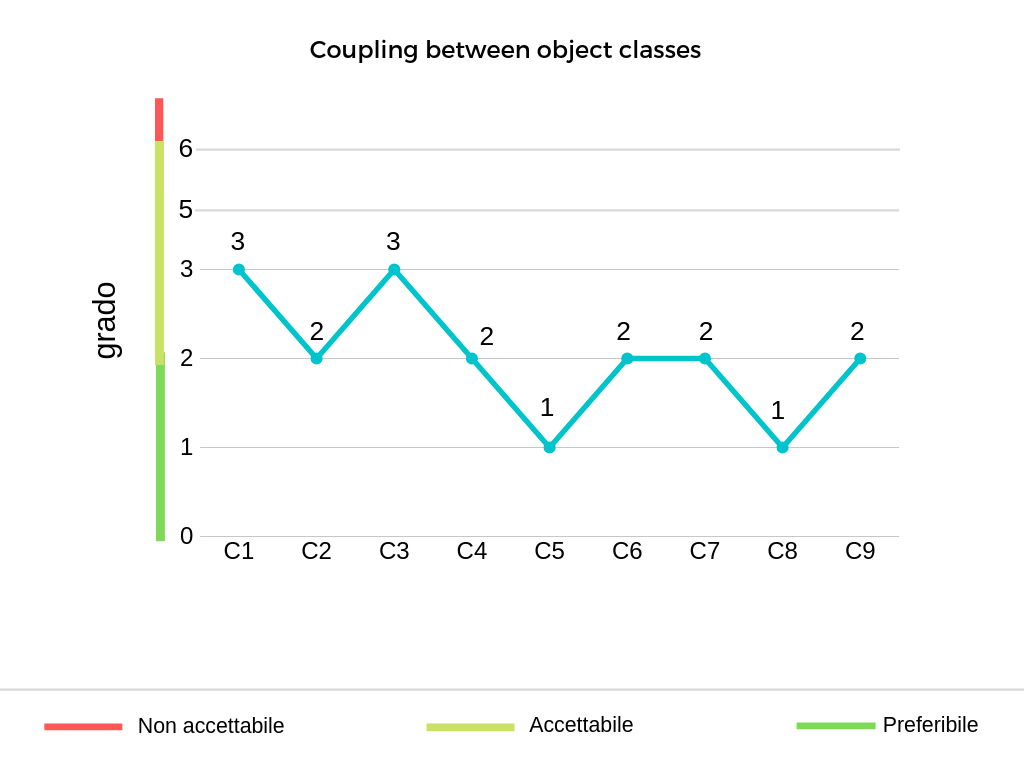
\includegraphics[width=0.90\textwidth]{res/images/new/cbo.png}\\
			\caption{Coupling Between Object classes}
		\end{figure}
	\end{center}
	\paragraph*{Valutazione} Le funzioni sviluppate in questo periodo presentano un buon grado di CBO. Le valutazioni sono molto vicine ai valori proferibili. \\ 
	La metrica è superata. 
	\pagebreak
	\subparagraph{Code coverage}
	\begin{center}
		\begin{figure}[h] 
			\centering 
			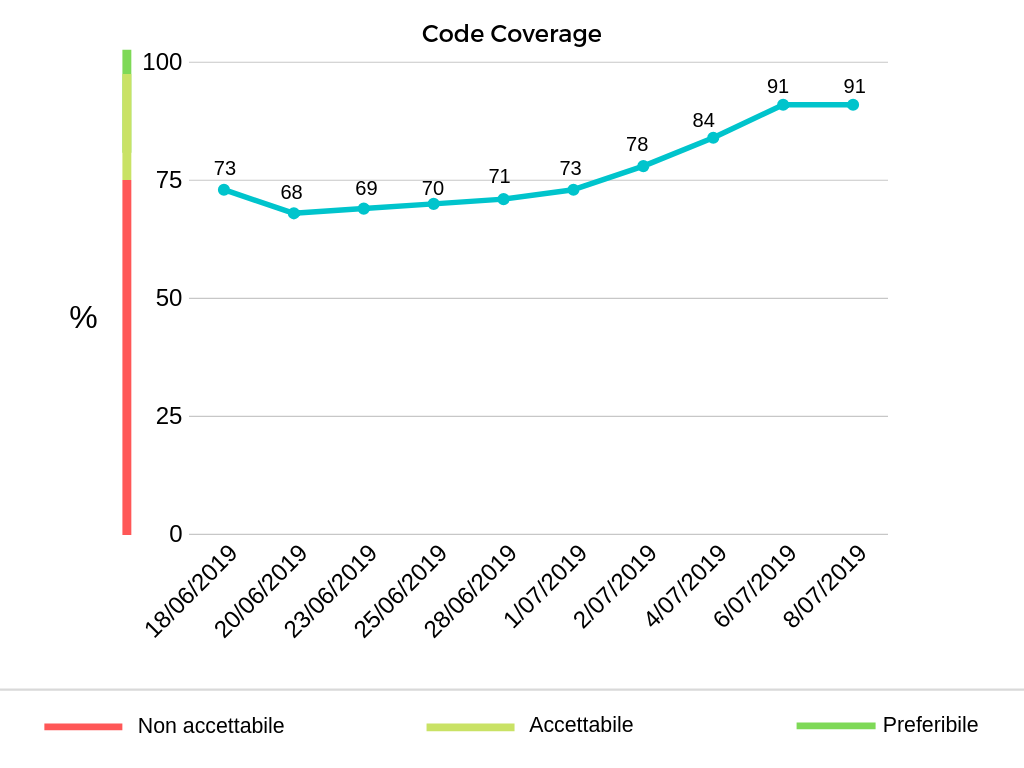
\includegraphics[width=0.90\textwidth]{res/images/new/codecov.png}\\
			\caption{Code coverage}
		\end{figure}
	\end{center}
	\paragraph*{Valutazione} All'inizio del periodo il code coverage era ad un livello insoddisfacente ma è stato poi colmato durante il periodo di sviluppo di test. Infatti da metà periodo il livello di code coverage aumenta, superando le richieste di accettazione, con andamento crescente verso i valori preferibili. \\
	La metrica è superata.
	\pagebreak
	\subparagraph{Indice Gunning fog}
	\begin{center}
		\begin{figure}[h] 
			\centering 
			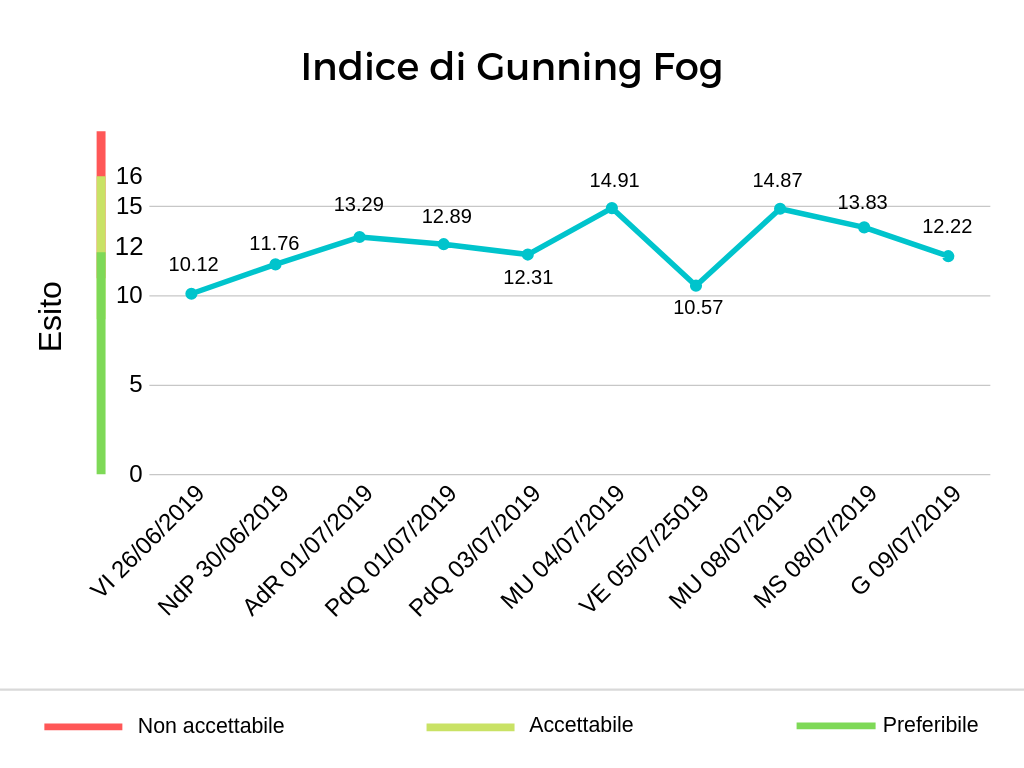
\includegraphics[width=0.90\textwidth]{res/images/new/gunningfog.png}\\
			\caption{Indice Gunning fog}
		\end{figure}
	\end{center}
	\paragraph*{Valutazione} In generale, nonostante l'impegno del gruppo nella semplificazione della sintassi, l'indice non sembra migliorare. Questo può  indicare una generale difficoltà nel semplificare documenti di natura tecnica. L'andamento della metrica è comunque soddisfacente, con valori intorno al valore preferibile. 
	Il documento \textit{Manuale utente} presenta dei valori leggermente più alti della norma, a causa dell'alto numero di immagini valutate male dallo strumento di verifica. 
	 \\
	La metrica è superata.
	\pagebreak
	\subparagraph{Indice di Gulpease}
	\begin{center}
		\begin{figure}[h] 
			\centering 
			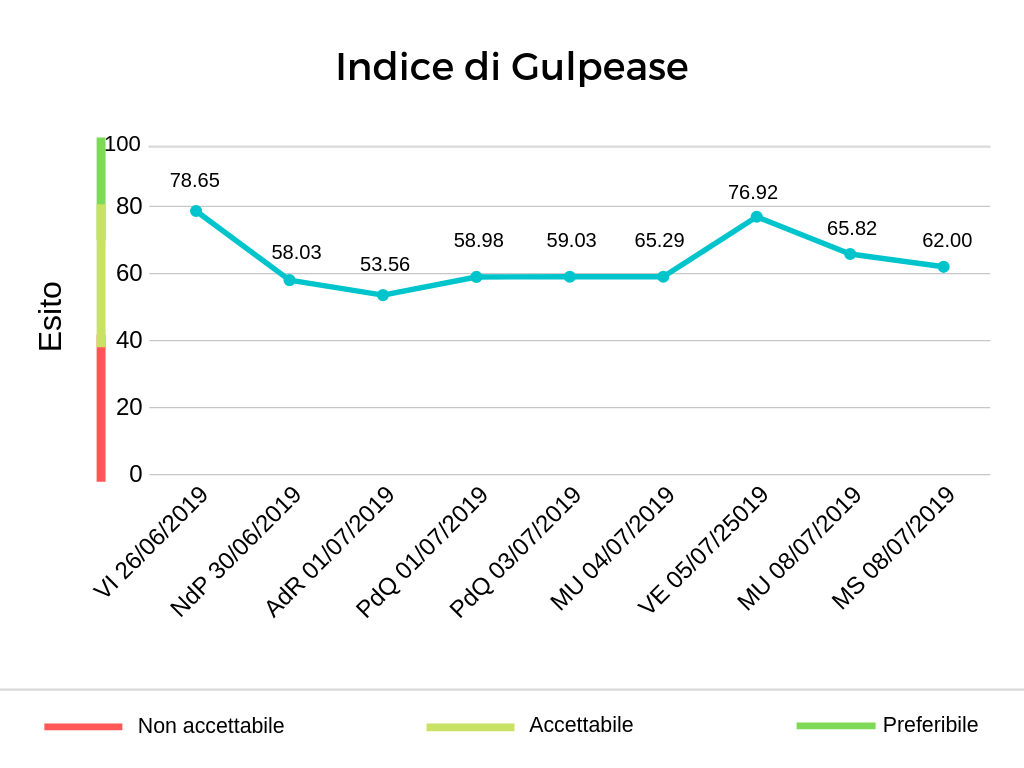
\includegraphics[width=0.90\textwidth]{res/images/new/gulpease.png}\\
			\caption{Indice di Gulpease}
		\end{figure}
	\end{center}
	\paragraph*{Valutazione} In generale, nonostante l'impegno del gruppo nella semplificazione della sintassi, l'indice non sembra migliorare. Questo può  indicare una generale difficoltà nel semplificare documenti di natura tecnica.
	A una valutazione posteriore, la soglia preferibile imposta appare eccessiva. La soglia di accettabilità invece è plausibile e rispettata.
	\pagebreak
	
		\paragraph{Qualità di prodotto}
		Di seguito viene riportata la misurazione delle metriche descritte in §3, derivanti dalla gestione di qualità di prodotto. \\
		Sono riportate in tabella le metriche di periodo e quelle che hanno avuto un valore costante nel tempo; la valutazione delle metriche rimanenti è riportata sotto forma di grafico a linea per evidenziarne la tendenza.
		\rowcolors{2}{pari}{dispari}	
	\begin{longtable}{ >{\centering}p{0.25\textwidth} >{\centering}p{0.10\textwidth}
			 >{\centering}p{0.10\textwidth} >{\centering}p{0.07\textwidth} >{\centering}p{0.31\textwidth}}
		\caption{  Valutazione della qualità di prodotto - RA} \\
		%\hline
		\rowcolorhead
		
		\centering\textbf{\color{white}Nome metrica} 
		& \centering\textbf{\color{white}Unità di misura} 
		& \centering\textbf{\color{white}Valore} 
		& \centering\textbf{\color{white}Esito}
		& \centering\textbf{\color{white}Accettazione}
		\tabularnewline %\hline 
		\endfirsthead
		
		\rowcolor{white}\caption[]{(continua)}\\	
		\rowcolorhead
		\centering\textbf{\color{white}Nome metrica} 
		& \centering\textbf{\color{white}Unità di misura} 
		& \centering\textbf{\color{white}Valore} 
		& \centering\textbf{\color{white}Esito}
		& \centering\textbf{\color{white}Accettazione}
		\tabularnewline %\hline 
		\endhead
		
		Requisiti obbligatori soddisfatti & \% & 100 & S & 100
		\tabularnewline
		
		Risoluzione dei guasti & \% & 100 & S & 100
		\tabularnewline
		
		Profondità della gerarchia & V & 3 & S & $ \leq 7 $
		\tabularnewline		
	\end{longtable}
	
	\subparagraph{Densità dei guasti nei casi di test}
	\begin{center}
		\begin{figure}[h] 
			\centering 
			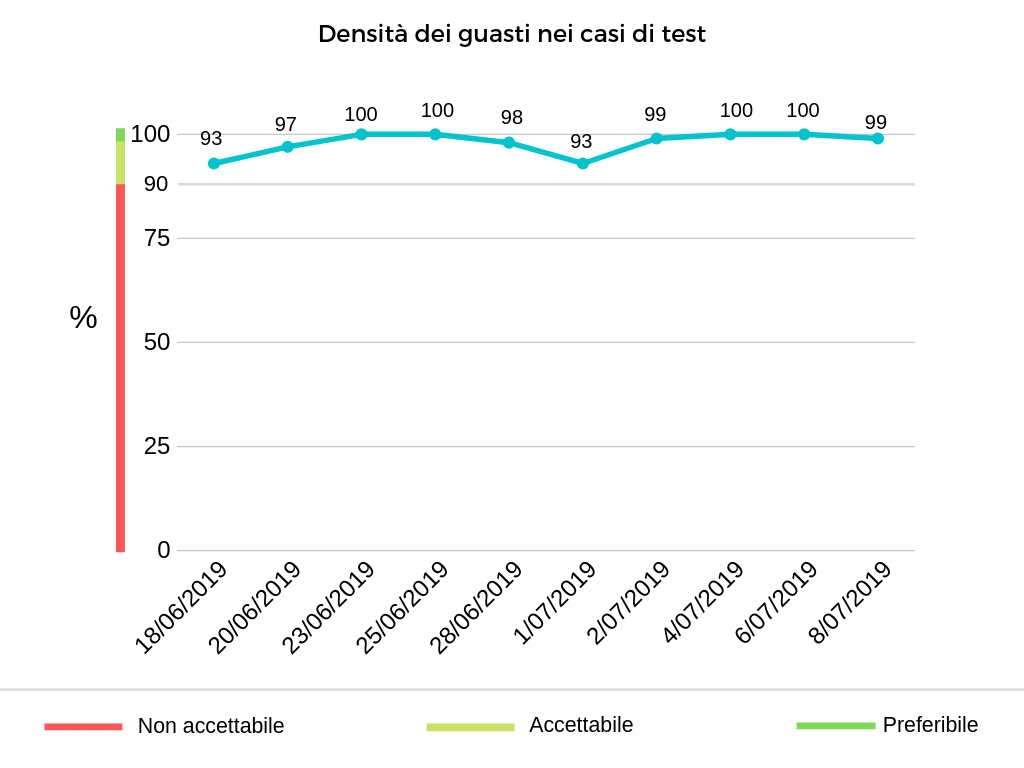
\includegraphics[width=0.90\textwidth]{res/images/new/densitaGuasti.png}\\
			\caption{Densità dei guasti nei casi di test}
		\end{figure}
	\end{center}
	\paragraph*{Valutazione} La metrica presenta  un buon andamento. È presente qualche picco verso il basso ma che è comunque contenuto. 
	\\
	La metrica è superata. 
	\pagebreak
	\subparagraph{Facilità di utilizzo}
	\begin{center}
		\begin{figure}[h] 
			\centering 
			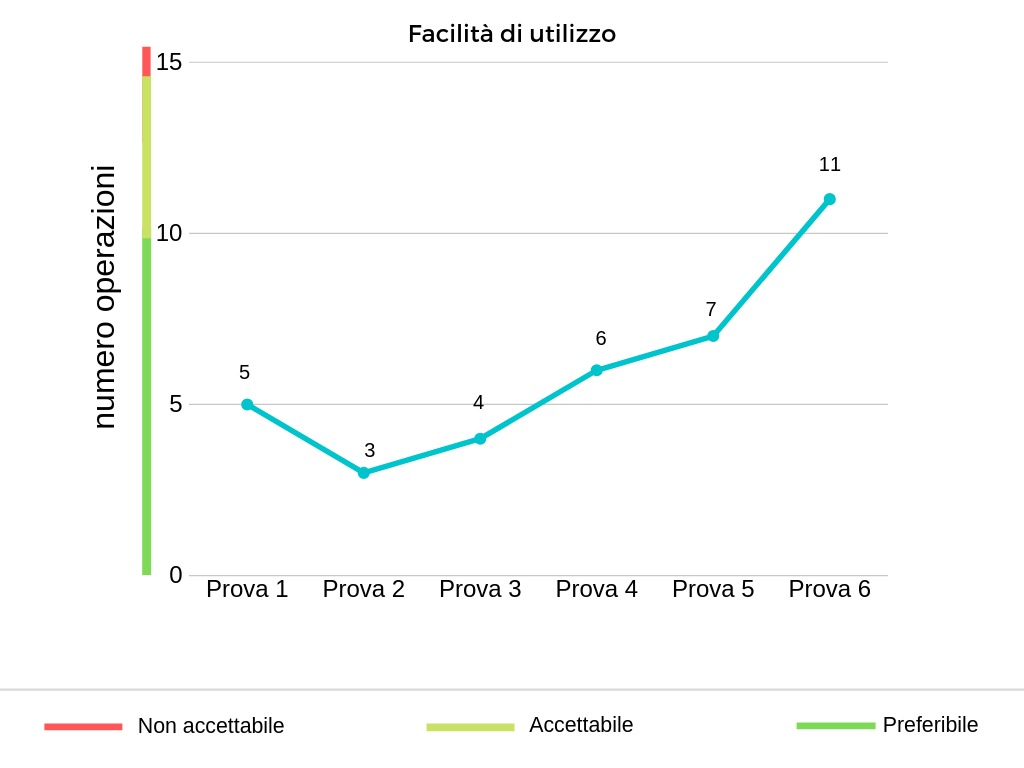
\includegraphics[width=0.90\textwidth]{res/images/new/facilitaUtilizzo.png}\\
			\caption{Facilità di utilizzo}
		\end{figure}
	\end{center}
	\paragraph*{Valutazione} La metrica ha un buon andamento, con valori tendenti all'ottimale. Solo una prova presenta un valore più alto del normale, la Prova 6 che riguarda la funzionalità di impostazione della disponibilità ripetuta dell'auto, dovuta al grande numero di operazioni richiesti ma che sono necessari. 
	\\
	La metrica è superata.
	\pagebreak
	\subparagraph{Facilità di apprendimento}
	\begin{center}
		\begin{figure}[h] 
			\centering 
			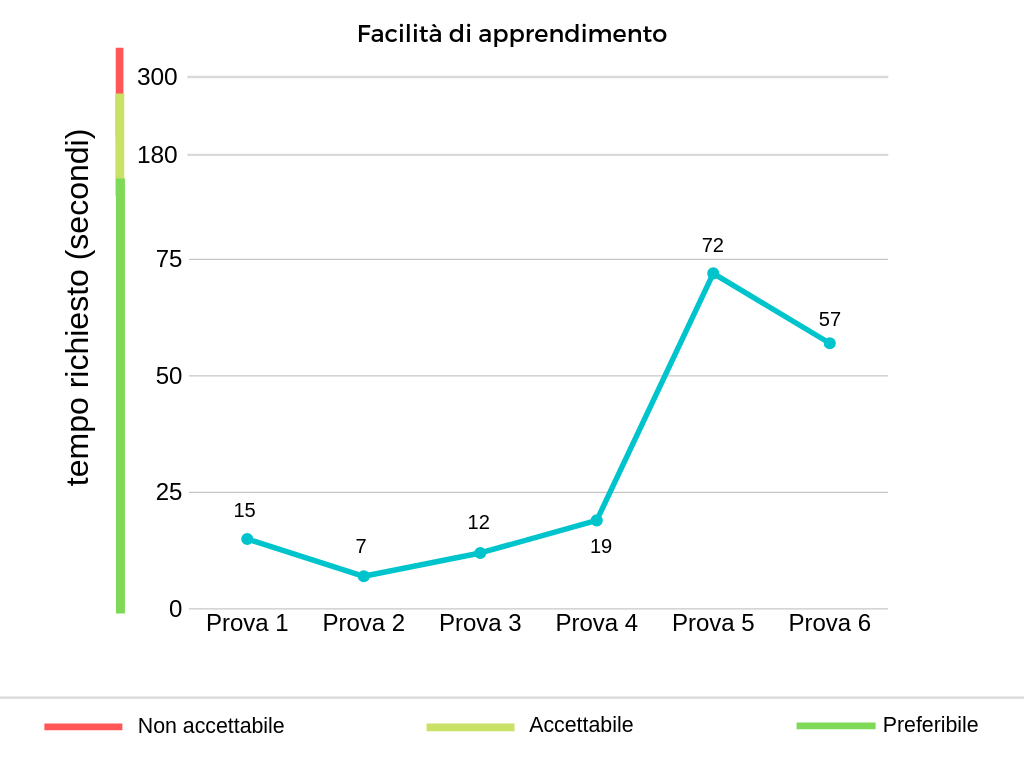
\includegraphics[width=0.90\textwidth]{res/images/new/facilitaApprendimento.png}\\
			\caption{Facilità di apprendimento}
		\end{figure}
	\end{center}
	\paragraph*{Valutazione} La metrica presenta un buon andamento. il picco più  alto della Prova 5 e' causato dalla funzionalità  di aggiunta disponibilità  ripetuta dell'auto, che non può  essere semplificata ulteriormente. A una valutazione posteriore il valore ottimale e il valore di accettazione risultano eccessivi. 
	\\ La metrica è superata.
	\pagebreak
	\subparagraph{Comprensione delle funzioni}
	\begin{center}
		\begin{figure}[h] 
			\centering 
			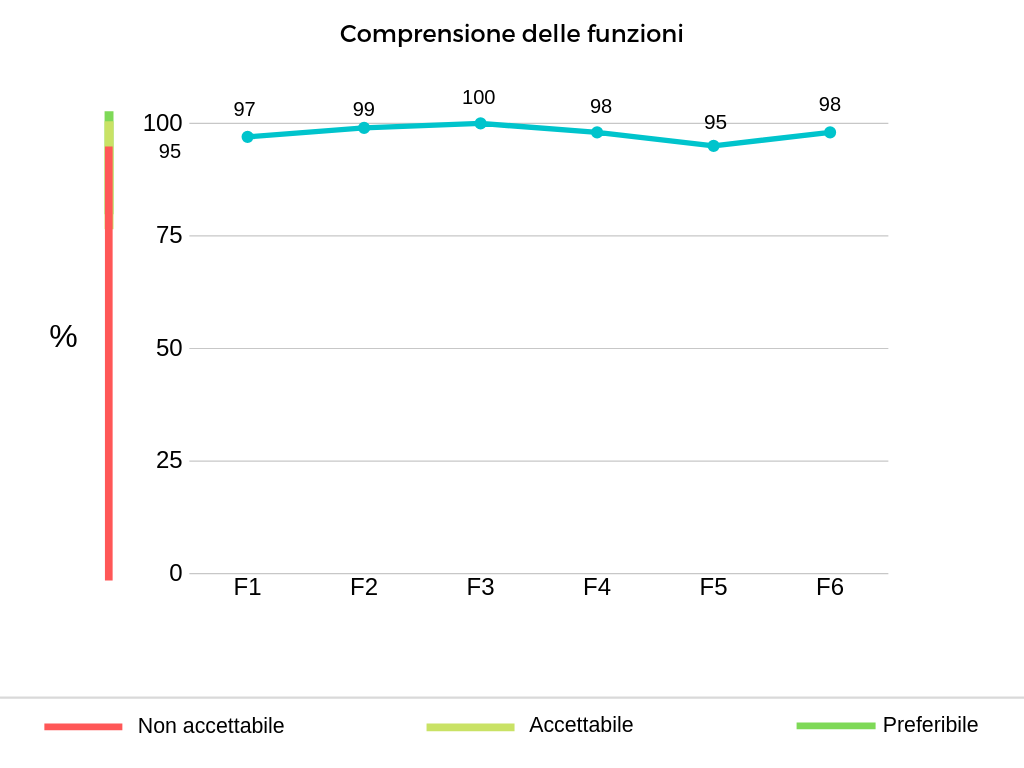
\includegraphics[width=0.90\textwidth]{res/images/new/comprensioneFunzioni.png}\\
			\caption{Comprensione delle funzioni}
		\end{figure}
	\end{center}
	\paragraph*{Valutazione} Il gruppo si è  impegnato a rendere le funzionalità più  intuitive migliorando l'interfaccia grafica e ha raggiunto dei buoni risultati, molto vicini al valore ottimale.
	\\ La metrica è superata.
	\pagebreak
	\subparagraph{Facilità di comprensione}
	\begin{center}
		\begin{figure}[h] 
			\centering 
			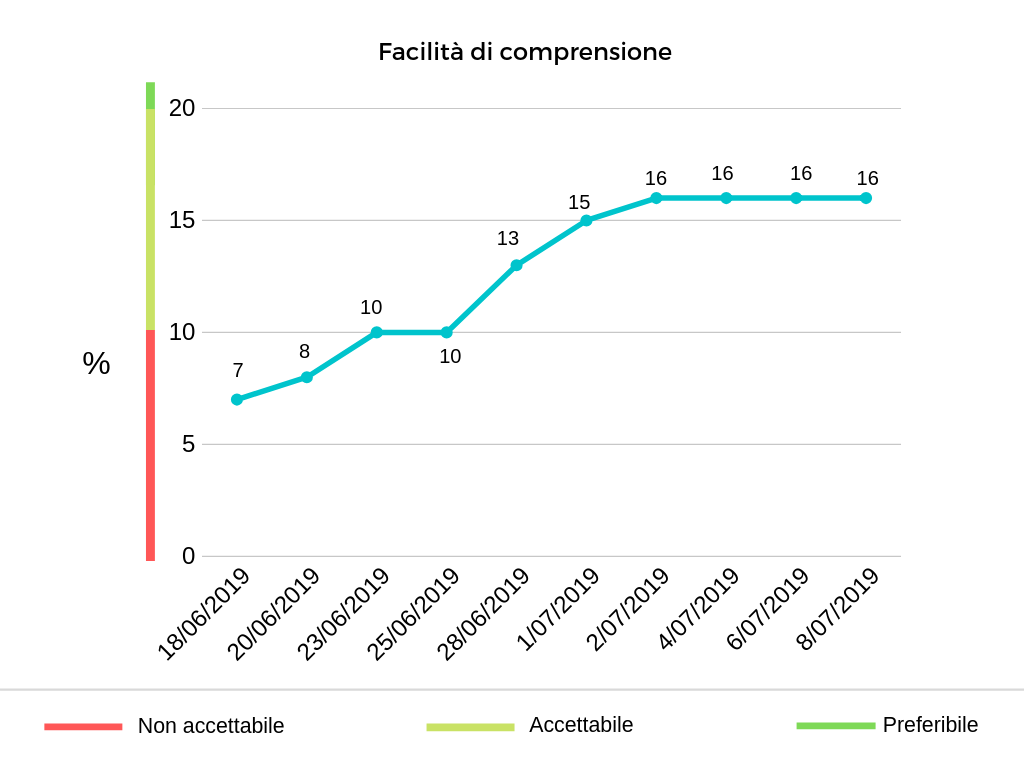
\includegraphics[width=0.90\textwidth]{res/images/new/facilitaComprensione.png}\\
			\caption{Facilità di comprensione}
		\end{figure}
	\end{center}
	\paragraph*{Valutazione} Inizialmente il livello della metrica era piuttosto basso. Successivamente il gruppo si è impegnato a migliorarla inserendo un gran numero di commenti, fino a raggiungere un buon livello tendente all'ottimo.
	\\ La metrica è superata.
	\pagebreak
	\subparagraph{Semplicità delle funzioni}
	\begin{center}
		\begin{figure}[h] 
			\centering 
			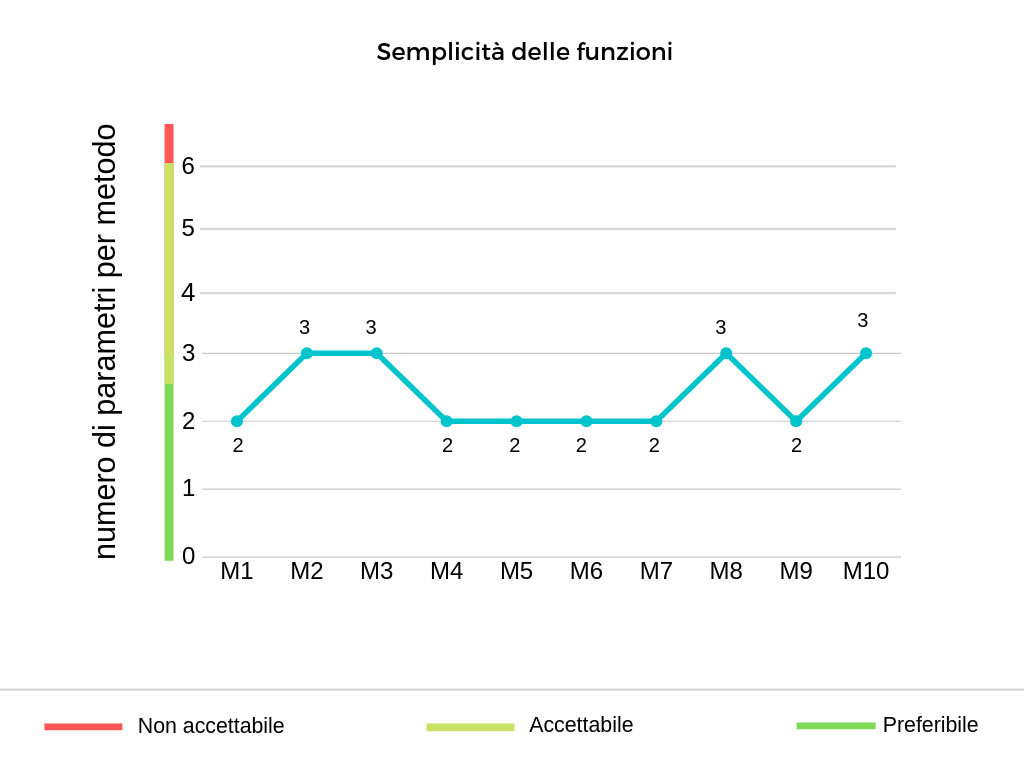
\includegraphics[width=0.90\textwidth]{res/images/new/semplicitaFunzioni.png}\\
			\caption{Semplicità delle funzioni}
		\end{figure}
	\end{center}
	\paragraph*{Valutazione} La metrica presenta un buon andamento in tutto il periodo. Ad una valutazione posteriore il limite di accettazione imposto appare troppo alto.
	\\ La metrica è superata.
	\pagebreak
	\subparagraph{Semplicità delle classi}
	\begin{center}
		\begin{figure}[h] 
			\centering 
			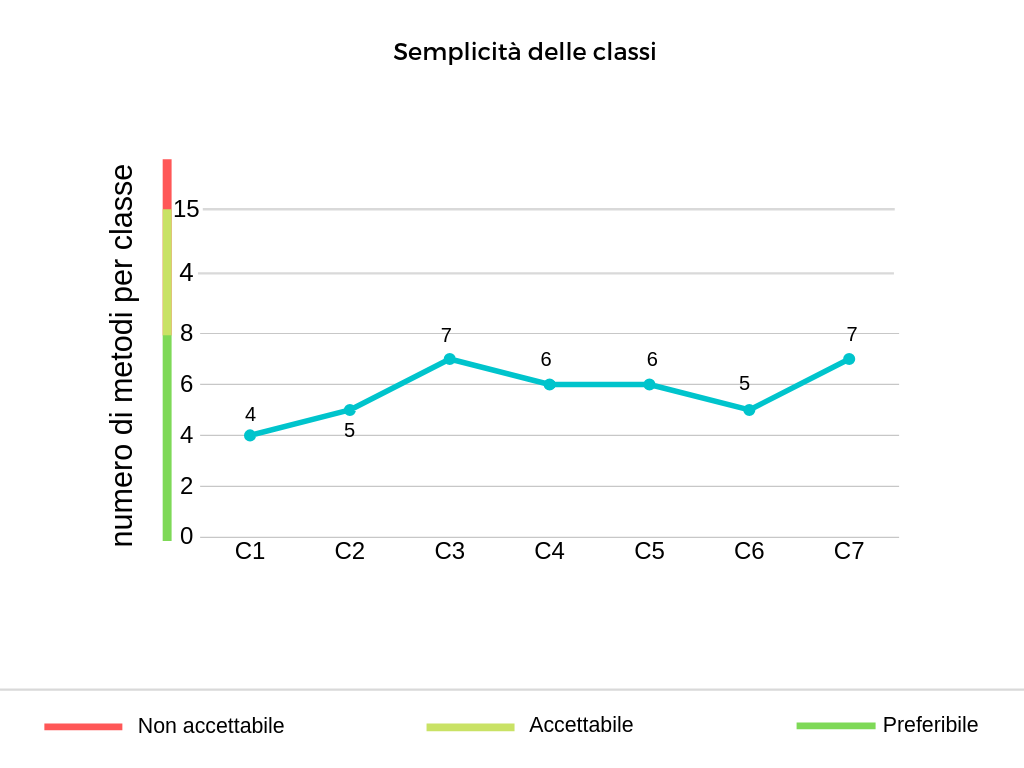
\includegraphics[width=0.90\textwidth]{res/images/new/semplicitaClassi.png}\\
			\caption{Semplicità delle classi}
		\end{figure}
	\end{center}
	\paragraph*{Valutazione} La metrica presenta un buon andamento con valori ottimali. Ad una valutazione posteriore il limite di accettazione imposto appare eccessivo. 
	\\ La metrica è superata.
	\pagebreak
	\subparagraph{SFIN: Structural Fan-in}
	\begin{center}
		\begin{figure}[h] 
			\centering 
			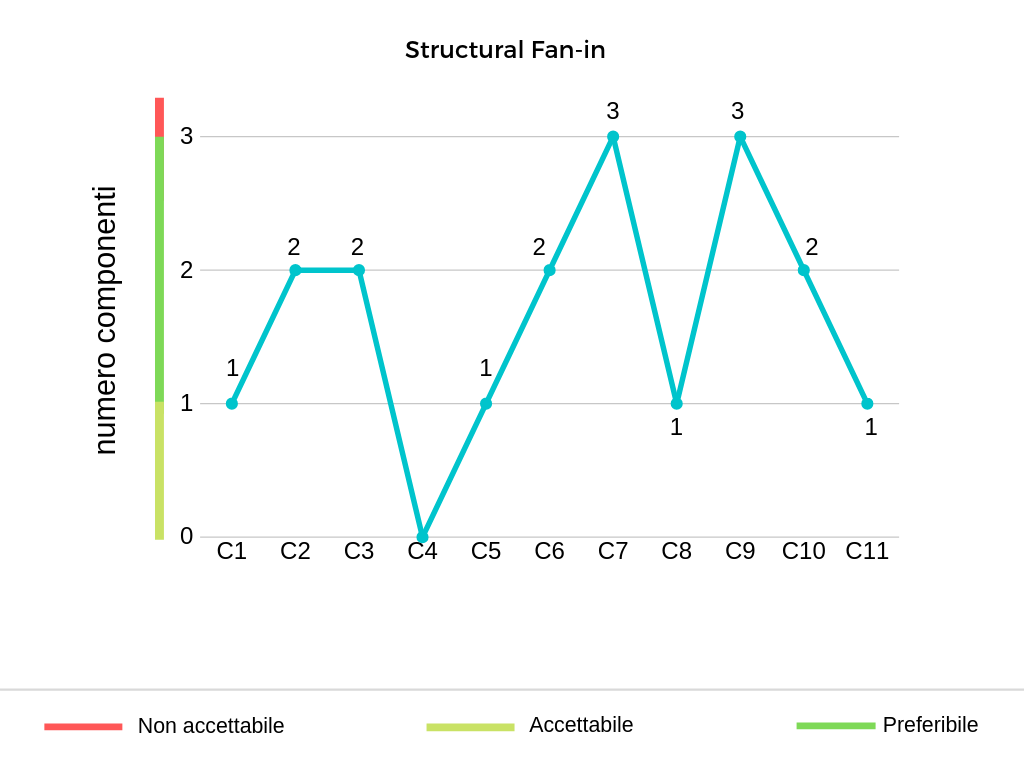
\includegraphics[width=0.90\textwidth]{res/images/new/sfin.png}\\
			\caption{SFIN: Structural Fan-in}
		\end{figure}
	\end{center}
	\paragraph*{Valutazione} La metrica presenta un andamento prevalentemente con valori accettabili. I valori riscontrati sono comunque molto discordanti, dovute al fatto che alcune funzionalità sono più complesse di altre.
	\\ La metrica è superata.
	\pagebreak
	\subparagraph{SFOUT: Structural Fan-out}
	\begin{center}
		\begin{figure}[h] 
			\centering 
			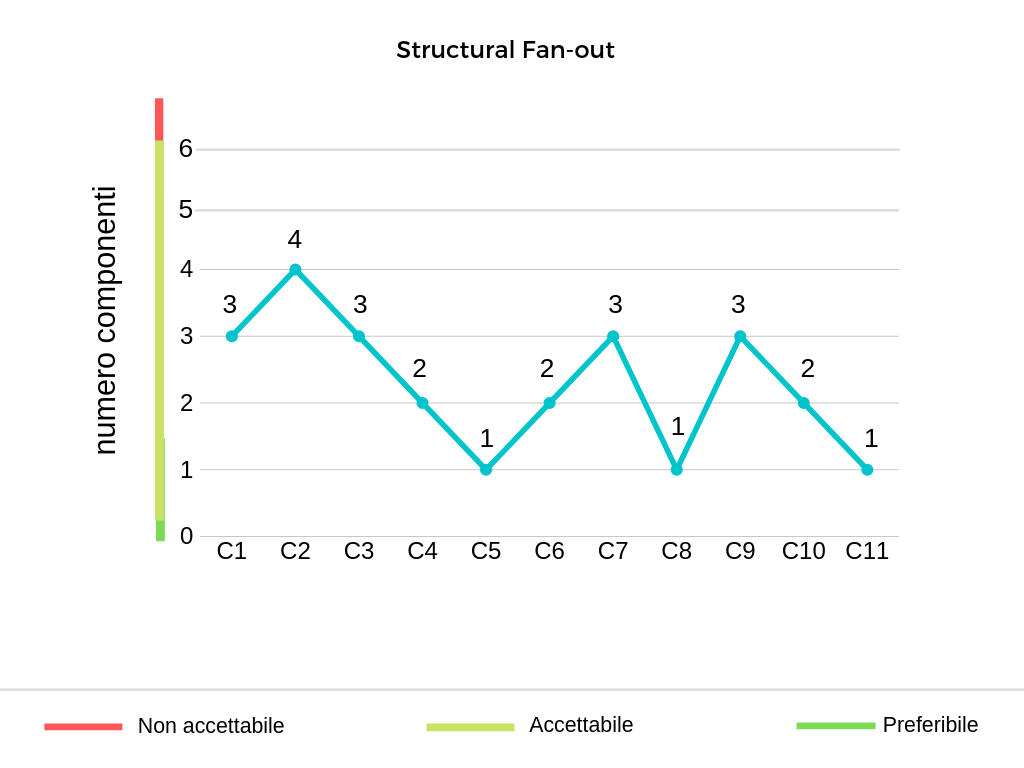
\includegraphics[width=0.90\textwidth]{res/images/new/sfout.png}\\
			\caption{SFOUT: Structural Fan-out}
		\end{figure}
	\end{center}
	\paragraph*{Valutazione} La metrica presenta valori accettabili, con valori che oscillano verso il margine ottimale.
	\\ La metrica è superata.
	\pagebreak

\paragraph{Esiti dei test - RA}

Di seguito viene riportata la tabella indicante l'esito dei test effettuati durante la fase di Revisione di Accettazione. Ogni test è stato eseguito più volte nel periodo, in base alle esigenze. Viene riportato solo l'esito finale.

\subparagraph{Test di unità}
Non sono stati aggiunti altri test di unità e non si è riscontrata la necessità di rieseguire i test già valutati.
\subparagraph{Test di integrazione}
Non sono stati aggiunti altri test di integrazione e non si è riscontrata la necessità di rieseguire i test già valutati.
\subparagraph{Test di sistema}
{\color{white}.}
\renewcommand{\arraystretch}{1.5}
\rowcolors{2}{pari}{dispari}

\begin{longtable}{ 			>{\centering}p{0.10\textwidth}
>{\centering}p{0.10\textwidth} >{\centering}p{0.10\textwidth} >{\centering}p{0.10\textwidth}
	}
	\caption{   Esito test di sistema - RA}\\	
	\rowcolorhead
	\textbf{\color{white}Test}
	& \textbf{\color{white}Requisito}  
	& \textbf{\color{white}N. prove} 
	& \textbf{\color{white}Esito finale}
	\tabularnewline 
	\endfirsthead	
	
	\rowcolor{white}\caption[]{(continua)}\\	
	\rowcolorhead
	\textbf{\color{white}Test} 
	& \textbf{\color{white}Requisito}
	& \textbf{\color{white}N. prove}
	& \textbf{\color{white}Esito finale}  
	\tabularnewline  
	\endhead	
	TS1&RFO2& 5 & Superato  \tabularnewline
	
	TS2&RFD1& 4 & Superato  \tabularnewline
	
	TS3&RFO3& 4 & Superato  \tabularnewline
	
	TS3.1&RFO2.7& 3 & Superato  \tabularnewline
	
	TS3.2&RFO3.3& 3 & Superato  \tabularnewline 
	
	TS4&RFO3.4& 5 & Superato  \tabularnewline
	
	TS5&RFO4& 4 & Superato  \tabularnewline
	
	TS6&RFO5& 4 & Superato  \tabularnewline
	
	TS6.1&RFO5.1& 3 & Superato  \tabularnewline
	
	TS6.2&RFO5.2\\RFO5.2.1\\RFO5.2.2\\RFO5.2.3& 4 & Superato  \tabularnewline
	
	TS7&RFO6\\RFO6.1& 5 & Superato \tabularnewline
	
	TS7.1&RFO6.2& 2 & Superato  \tabularnewline
	
	TS7.2&RFO6.3& 3 & Superato  \tabularnewline
	
	TS7.3&RFO6.4& 4 & Superato  \tabularnewline
	
	TS7.4&RFO6.5& 4 & Superato  \tabularnewline
	
	TS7.5&RFO6.6& 2 & Superato  \tabularnewline
	
	TS8&RFO7\\RFO7.1\\RFO7.2\\RFO7.3\\RFO7.4\\RFO7.5& 5 & Superato \tabularnewline
	
	TS9&RFD8& 6 & Superato  \tabularnewline
	
	TS10&RFO9& 5 & Superato  \tabularnewline
	
	TS10.1&RFO9.2& 6 & Superato  \tabularnewline
	
	TS10.1.1&RFO9.1& 3 & Superato  \tabularnewline
	
	TS10.1.2&RFO9.2.8& 4 & Superato  \tabularnewline
	
	TS10.2&RFO9.3& 4 & Superato  \tabularnewline
	
	TS11&RFF10& 4 & Superato  \tabularnewline
	
	TS11.1&RFF10.1& 2 & Superato  \tabularnewline
	
	TS11.1.1&RFF10.1.1\\RFF10.1.2& 5 & Superato  \tabularnewline
	
	TS11.2&RFF10.2& 3 & Superato  \tabularnewline
	
	TS11.2.1&RFF10.2.1\\RFF10.2.2& 6 & Superato  \tabularnewline
	
	TS11.3&RFF10.3& 2 & Superato  \tabularnewline
	
	TS11.3.1&RFF10.3.1& 4 & Superato  \tabularnewline
	
	TS11.4&RFF10.4& 4 & Superato  \tabularnewline
	
	TS11.4.1&RFF10.4.1\\RFF10.4.1.1& 6 & Superato  \tabularnewline
	
	TS12&RFF11& 3 & Superato  \tabularnewline
	
	TS13&RFF2.6& 5 & Superato  \tabularnewline
	
	TS14 &RFF12& 4 & Superato  \tabularnewline
	
	TS14.1&RFF12.1& 6 & Superato  \tabularnewline
	
	TS14.2&RFF12.2& 5 & Superato  \tabularnewline
	
\end{longtable}		
